\documentclass[12pt]{article}
\usepackage[latin9]{inputenc}
\usepackage{microtype}
\usepackage[letterpaper]{geometry}
\geometry{verbose,tmargin=1in,bmargin=1in,lmargin=1in,rmargin=1in}
\pagestyle{plain}
\usepackage{color}
\usepackage{float}
\usepackage{amsmath}
\usepackage{amssymb}
\usepackage{graphicx}
\usepackage[authoryear]{natbib}
\usepackage{chngcntr}
\usepackage{subcaption}

%%%%%%%%%%%%%%%%%%%%%%%%%%%%%%  SPACING
\usepackage{setspace}

\onehalfspacing % working paper spacing

%\doublespacing % journal submission spacing
%\usepackage{footmisc} % journal submission spacing
%\renewcommand{\footnotelayout}{\doublespacing} % journal submission spacing
%%%%%%%%%%%%%%%%%%%%%%%%%%%%%% 

\usepackage[unicode=true,
 bookmarks=false,
 breaklinks=false,pdfborder={0 0 1},backref=false,colorlinks=false]
 {hyperref}
\usepackage{breakurl}

\makeatletter

%%%%%%%%%%%%%%%%%%%%%%%%%%%%%%  PACKAGES FOR COMMENTING
% USER WRITTEN COMMENT COMMAND

% IF SELECTED, COMMAND WILL NOT DISPLAY COMMENTED TEXT  
%\newcommand{\comment}[1]{}  %comment not shown

%IF SELECTED, COMMAND WILL PRINT COMMENTED TEXT IN BLUE  
\newcommand{\comment}[1]
{{\bfseries \color{red} #1}} %comment shown

%%%%%%%%%%%%%%%%%%%%%%%%%%%%%% User specified LaTeX commands.
\setcounter{MaxMatrixCols}{10}

\usepackage{booktabs}% Pretty tables
\usepackage{tabularx}% 
\usepackage{threeparttable}% For Notes below table

\usepackage{amsfonts}
\usepackage{multicol}
\usepackage{lscape}
\usepackage{rotating}

\usepackage{changepage}
\usepackage{pdfpages}
\usepackage{geometry}
\usepackage{graphicx}

\usepackage{xcolor}
\hypersetup{
    colorlinks,
    linkcolor={blue!80!black},
    citecolor={blue!80!black},
    urlcolor={blue!80!black}
}

%PUT DATE IN MONTH-YEAR
\usepackage{datetime}
\newdateformat{monthyeardate}{%
  \monthname[\THEMONTH] \THEYEAR}
\makeatother

\begin{document}

\title{Investment versus Output Subsidies: Implications of Alternative Incentives for Wind Energy}

\author{Joseph E. Aldy, Todd D. Gerarden, and Richard L. Sweeney\thanks{\protect Aldy: Harvard Kennedy School, Resources for the Future, National Bureau of Economic Research, and Center for Strategic and International Studies; \protect\href{mailto:joseph_aldy@hks.harvard.edu}{joseph\_{}aldy@hks.harvard.edu}. Gerarden: Cornell University; \protect\href{mailto: gerarden@cornell.edu}{ gerarden@cornell.edu};
Sweeney: Boston College; \protect\href{mailto:sweeneri@bc.edu}{sweeneri@bc.edu}. \newline \protect\hphantom{} \hspace{3ex} Data and code for replication are available at \protect\href{https://github.com/rlsweeney/public_ags_output_subsidies}{https://github.com/rlsweeney/public\_ags\_output\_subsidies}. \newline \protect\hphantom{} \hspace{3ex} Blake Barr, Juliet Bramante, Jeff Bryant, Napat Jatusripitak, Ken Norris, Michael O'Brien, Carlos Paez, Jun Shepard, Avi Zevin, and Howard Zhang provided excellent research assistance. Thanks to Scott Walker, Gabe Chan and Joern Huenteler for assistance with wind speed data; and Curtis Carlson, John Horowitz, and Adam Looney for assistance with historical tax policy information. This project has been supported by the Alfred P. Sloan Foundation (grant 2015-13862) and the Harvard University Center for the Environment. Aldy acknowledges support from BP, the Taubman Center, and the Belfer Center. Gerarden acknowledges support from U.S. EPA STAR Fellowship no. FP-91769401-0. We have benefited from feedback provided at several conferences; by seminar attendees at Chicago, Columbia, Duke, Harvard, LSE, Oxford, UAlbany, and Pitt; as well as from Alberto Abadie, Lucas Davis, Kelsey Jack, Jud Jaffe, Ken Gillingham, Justin Kirkpatrick, Joel Landry, Jeff Liebman, Erin Mansur, Paul Goldsmith-Pinkham, Matt Rogers, Dick Schmalensee, Jim Stock, and Martin Weitzman. }}


\date{\monthyeardate\today}
\maketitle
\begin{abstract}
\noindent This paper examines the choice between subsidizing investment and subsidizing output to promote socially desirable production. We exploit a natural experiment to estimate the impact of subsidy margin on the productivity of wind farms. Using instrumental variable and matching estimators, we find that investment subsidy claimants produce \input{../output/estimates/stat_rd_estimate_pct.tex} \unskip to \input{../output/estimates/stat_match_estimate_pct.tex}percent less power than they would have under the output subsidy. Accounting for extensive margin effects, we show that output subsidies are more cost-effective than investment subsidies over a large range of output targets. 

\vspace{1cm}

\noindent Keywords: tax credits, energy subsidies, instrument choice

\noindent JEL Codes: H23, Q42, Q48

\vspace{1cm}
\end{abstract}

\pagebreak
\section{Introduction}

Governments subsidize investment for a variety of reasons. When economic output falls well below potential output, policymakers subsidize investment to stimulate the economy. To address the market failure of innovation spillovers, governments subsidize research and development spending. To increase the supply of affordable housing, governments subsidize low-income housing development. To spur the replacement of pollution-intensive facilities, policymakers subsidize the construction of low-emission power plants. In each of these examples, the social benefits of subsidized investments are tied to the eventual \textit{output} they produce, not just the investment itself. Given this, it is noteworthy that governments also often \textit{directly} subsidize output in each of these settings, through government procurement, research prizes, housing vouchers, and tax credits for clean energy production. 

Is it better to subsidize investment or output? If the government's objective is to minimize the public expenditure necessary to meet an output target, the answer is theoretically ambiguous. Whether investment subsidies are more or less cost-effective than output subsidies depends on how intensively investment goods are used on the margin, compared to on average, and how substitutable they are with other unsubsidized inputs \citep{parish_relative_1982}. Despite the ubiquity of both types of subsidies, there is little empirical evidence comparing their cost-effectiveness in practice. 

In this paper, we provide the first direct empirical evidence on this topic. We focus on the U.S. wind power industry, where a unique policy innovation introduced through the American Recovery and Reinvestment Act of 2009 temporarily allowed project developers to choose between investment and output subsidies. Before January 1, 2009, wind farm developers could only claim the Production Tax Credit (PTC), equal to \$23 per megawatt-hour (MWh) for the first ten years of output. From 2009 to 2012, developers could choose between the PTC and the Section 1603 grant, an upfront cash payment equal to 30 percent of investment costs. We leverage this natural experiment to compare the relative cost-effectiveness of these investment and output subsidies using three sets of complementary analyses. 

First, we focus on the intensive margin and find that plants claiming the investment subsidy were \input{../output/estimates/stat_rd_estimate_pct.tex} \unskip to \input{../output/estimates/stat_match_estimate_pct.tex}percent less productive than they would have been under the output subsidy.\footnote{As we discuss in Section \ref{subsec:outputModel}, the different subsidies lead to different levels of output through two channels: (1) differences in wind farm downtime and ``availability'' to produce, and (2) differences in the probability that a wind farm will be selected by the grid operator to produce, conditional on being available. Although we lack the data to decompose our productivity estimates along these lines, we discuss the efficiency implications of the two mechanisms in Section \ref{sec:Mechanism}.} These estimates reflect two empirical strategies that rely on different identifying assumptions. Since there is no within-plant variation in subsidy type, we compare the output of plants that selected the investment subsidy with those that selected the output subsidy. As one approach to address concerns about this selection, we restrict the sample to wind farms placed into service within 12 months of the January 1, 2009 policy change. Within this window, the long lead time of wind farm development ensures that all siting and capital decisions would have been fixed well before the 1603 program was even conceived. To estimate the effect of replacing output with investment subsidies, we instrument for investment subsidy selection with an indicator for whether a plant was eligible for the 1603 grant.\footnote{We also use this instrument for a parametric fuzzy regression discontinuity design in Appendix Table~\ref{tab:rdd_cf_linear}.} For our second approach, we use a matched difference-in-differences estimator on the full population of wind farms placed into service between 2005 and 2012. We employ matching to identify those plants in the pre-2009 period that would have selected the investment subsidy had the 1603 grant been available. We compare output between plants that, based on observables, appear to prefer output subsidies to those that appear to prefer investment subsidies before and after investment subsidies were made available.

Second, we evaluate the extensive margin gains associated with the introduction of the 1603 grant program and assess whether they could offset these intensive margin production losses. Long project lead times coupled with the short duration of the program limited the set of potential entrants to projects already in the development process when Congress unexpectedly legislated the program. Using more than a decade of data on wind farm proposals, we find little change in the probability that a proposed plant comes to fruition during the 1603 grant program period. In order to estimate how many proposed wind farms were ``saved'' by the grant program following the financial crisis, we use plant-specific investment cost and marginal revenue data to construct each plant's expected discounted lifetime profits, and find that only \input{../output/estimates/pe_baseline_pi-1603-only_Pct.tex} \unskip percent of the 1603 recipients appear marginal to the investment subsidy. Accounting for both intensive and extensive margin impacts, we estimate that the 1603 program reduced total wind output among recipients by \input{../output/estimates/pe_baseline_Always_dQ_diff_pct.tex} \unskip percent, while \emph{increasing} the total public cost by \input{../output/estimates/pe_baseline_Always_C_diff_pct.tex} \unskip percent.

Third, we use these analyses to generate commensurable estimates of the public expenditure required to achieve a given quantitative renewable energy target under each regime. This allows us to make direct comparisons of investment and output subsidies over a large range of output targets. For example, focusing solely on the population of plants selecting the 1603 grant, we find that the amount of wind power produced by a 30 percent investment subsidy could have been achieved at $\input{../output/estimates/ce_1603equivalentPTC_plcoe_pct.tex}$ percent lower cost using an output subsidy. We then extend the analysis to include all wind farms entering between 2009 and 2012, and remove the ability for wind developers to choose between subsidies. This further strengthens the case for an output subsidy, as costs are now lower than the investment subsidy at most quantity targets even if the intensive margin productivity response is ignored. 

Despite extensive research on both optimal taxation and instrument choice, there is little research on the relative performance of input and output subsidies.\footnote{The question was qualitatively discussed in several contexts in the 1980s. For example, \cite{stiglizWB1987} compares and contrasts crop price supports and fertilizer subsidies. \citet{schmalensee_appropriate_1980} considers the conceptual merits of government policy to increase energy production generally, and concludes that input subsidies build in ``potentially huge inefficiencies'' relative to an output subsidy.} There is a large literature on the effects of investment tax incentives across industries \citep[e.g.,][]{goolsbee_investment_1998,goolsbee_taxes_2004,house_temporary_2008}, but these papers do not compare investment incentives to alternative instruments that target output. A few relevant papers estimate dynamic structural models of \textit{adoption} in the solar industry \citep{burr2016subsidies,de_groote_subsidies_2019} or ethanol plant entry \citep{yi2018dynamic} in the presence of one of the two subsidies, and assess the impact of the other subsidy using counterfactual simulations. In contrast, we observe firms exposed to both types of subsidy simultaneously in the data, and exploit a natural experiment to directly compare outcomes across them. 

This paper also contributes to a growing literature on renewable energy policy. Several papers focus on estimating the environmental benefits of renewable electricity generation \citep[e.g.,][]{cullen_measuring_2013,novan_valuing_2015,callaway_location_2018,fell_emissions_nodate}. While we are primarily concerned with cost-effectiveness, we discuss the efficiency implications of different subsidy margins in section \ref{sec:Mechanism}. \citet{metcalf_investment_2010} relates the PTC to the user cost of capital and finds that wind investment is highly responsive to changes in tax policy. \citet{schmalensee_evaluating_2012} compares U.S. renewable subsidies to policy alternatives such as a feed-in tariff or a cap-and-trade program to limit emissions. Our paper is the first to study the impact of the incentives created by renewable subsidies on firm productivity. As such, we build upon prior work that showed electricity restructuring incentivized fossil fuel and nuclear power plants to operate more efficiently \citep[e.g.,][]{fabrizio_markets_2007,davis_deregulation_2012,cicala_when_2015}.

Finally, \cite{johnston_nonrefundable_2019} also studies the 1603 grant program. \citeauthor{johnston_nonrefundable_2019} focuses on the non-fungibility of the PTC and asks whether replacing it with a refundable tax credit or grant would increase wind power investment. Leveraging an identification approach similar to our IV strategy, \citeauthor{johnston_nonrefundable_2019} finds that wind farm developers value each PTC dollar at \$0.85. Crucially, the estimation approach used in that paper assumes the difference in marginal incentives between the PTC and 1603 grant has no impact on wind farm productivity. In contrast, we estimate the impact of these marginal incentives and find that they are large.

The rest of this paper proceeds as follows. Section~\ref{sec: Background} provides a brief introduction to the economics of wind energy, a summary of the policy environment, and a discussion of how production incentives differ under investment and output subsidies. Section~\ref{sec:Data} describes the data. Section~\ref{sec:Empirical-Strategy} summarizes the empirical strategy and results for our intensive margin analysis. Section~\ref{sec:Discussion} discusses our extensive margin and cost-effectiveness analyses as well as efficiency implications. Section~\ref{sec:Conclusion} concludes.

\section{Background \label{sec: Background}}

\subsection{The Economics of Wind Power \label{subsec:WindEcon}}

A wind turbine consists of a rotor with three long blades connected to a gearbox and generator atop a large tower. As wind passes through the blades, the rotor spins a drive shaft connected through a series of gears to a generator that converts this kinetic energy to electrical energy. The amount of power generated by a wind turbine is determined primarily by the design of the turbine and the velocity of the wind. Nameplate capacity, denominated in megawatts (MW), is the maximum rated output of a turbine operating in ideal conditions. Wind turbines typically operate at rated capacity at wind speeds of 33 miles per hour (15 meters/second), and shut down when the wind speed exceeds 45-55 miles per hour (20-25 meters/second) to prevent damage. Figure~\ref{fig:GE-powercurve} presents the marketed power curves for two common wind turbine models in our sample, demonstrating the nonlinear relationship between wind speed and output.

Building a wind farm involves large upfront costs. The average implied investment cost for plants receiving a 1603 grant in our data is \$165 million. Wind farm development also requires long lead times. Developers first have to survey and secure access to land that is both sufficiently windy and close to existing transmission lines. They then have to obtain financing and siting permits, as well as negotiate any power purchase agreements. The construction phase of a wind farm takes 9 to 12 months, with site permitting and turbine lead times often double that \citep{brown_arra_2011}. Turbines are ordered up to 24 months before ground is broken, and, at that point, the size and location of a project is essentially fixed.\footnote{Even during normal times, there is a natural lag between turbine contract signing and installation. But turbine lead times approached two years during the peak demand period in the first half of 2008 \citep[p. 12]{lantz_iea_2012}.} For wind farms coming online in 2009 and 2010 in the Midcontinent Independent System Operator (MISO), an average of 2.7 and 3.5 years passed between when the wind farms began the process of connecting to the grid and when they actually began supplying electricity.\footnote{Authors' estimate based on MISO interconnection queue data. New electricity generators enter the interconnection queue to request the ability to connect to the electricity grid and supply electricity once construction is complete.}

Although wind operators do not incur fuel costs, there are a number of variable costs associated with running a wind farm efficiently once it is installed. Turbines need to be monitored and serviced regularly to operate at peak efficiency \citep{wiser_2013_2014}. Placing more emphasis on routine maintenance can reduce the probability of failure, and, conditional on failure, service arrangements and crane availability induce variation in turnaround times across operators. The gearbox, in particular, contains a complicated set of parts that, if not serviced, can reduce the fraction of wind power harnessed or cause the unit to be taken offline entirely. In 2013, operations and maintenance (O\&M) costs at U.S. wind farms were on the order of \$5 to \$20 per MWh, with a few plants with O\&M costs in excess of \$60 per MWh \citep{wiser_2013_2014}.

\subsection{Wind Power Policies \label{subsec:RenewablePolicies}}

The United States has implemented policies to promote investment in wind power at the Federal, state, and local levels. Since 1992, the leading Federal subsidy for wind farm developers has been the PTC. The PTC is a tax credit for electricity generated by qualified energy resources and sold to an unrelated party during the tax year. A qualifying generation source can claim the PTC for the first ten years of generation after the plant is placed into service. Congress initially set the PTC at \$15/MWh, but automatic inflation adjustments made it worth \$23/MWh in 2014. Prior to the 2008 financial crisis, wind farm developers typically monetized tax credits by partnering with a financial firm in the tax equity market. During the financial crisis, more than half of the suppliers of tax equity exited this market. This introduced financing challenges for wind farm developers without sufficient tax liability to monetize the tax credits on their own \citep{u.s._pref_prospective_2010}.

In this financial context, wind farm developers sought new ways to realize the value of the PTC. In early January 2009, Congressional staffers and Presidential Transition Team members discussed for the first time the possibility of allowing large-scale wind power sources to receive an upfront cash grant worth 30 percent of investment costs in lieu of the PTC as part of what would become the American Recovery and Reinvestment Act of 2009 (``The Recovery Act'').\footnote{One of the authors served as one of two staff who negotiated the energy provisions of the Recovery Act representing the Obama Presidential Transition Team. He met regularly with staff to the House Ways and Means and Senate Finance Committees in December 2008 and January 2009, as well as with career Treasury staff in the Office of Tax Policy. In January 2009, upon agreement with Congressional negotiators of what became the Section 1603 grant in the Recovery Act, the author briefed a large meeting of the renewables industry at the Presidential Transition Team offices where the unexpected, novel nature of this policy was evident in the meeting participants' reactions.} When the bill became law the following month, Congress made this Section 1603 grant option available retroactively to projects placed into service on or after January 1, 2009. A wind project could claim a 1603 grant if it was placed into service between January 1, 2009 and December 31, 2012.\footnote{Technically, the December 2010 tax law extended the 1603 grant sunset date from December 31, 2010 to December 31, 2012.} Wind farms remained eligible for the PTC under existing law, and the Recovery Act extended the wind PTC until December 31, 2012 (before it was extended again by subsequent legislation). The Recovery Act thus provided wind power developers with a new, mutually exclusive subsidy choice: they could claim the PTC over 10 years or they could claim an upfront cash payment equal to 30 percent of eligible investment costs.\footnote{While the Recovery Act also provided developers with the option of taking the ITC, in practice, they chose between the PTC and the Section 1603 grant. The annual Internal Revenue Service Estimated Data Line Counts reports show that not one corporation claimed the ITC for a wind power project over 2009-2011.} In total, the Treasury made about 400 Section 1603 grant awards to large wind farms, disbursing over \$12 billion.

These two Federal subsidies were not the only policies affecting wind farms during the time period we study. There were other, overlapping regulatory and fiscal policy instruments focused on wind power development at the state and Federal levels, including accelerated depreciation and loan guarantees \citep{aldy_preliminary_2013,metcalf_investment_2010,schmalensee_evaluating_2012}. Many states also have a renewable portfolio standard (RPS) that mandates a minimum share of the state's power comes from renewable sources, resulting in a price premium for wind power. Under some state RPS programs, renewable energy certificates (RECs) for wind power generation have been worth more than \$50/MWh, or more than twice the value of the PTC \citep{schmalensee_evaluating_2012}. States also provide subsidies through state tax credits and property tax exemptions. For purposes of the statistical analyses below, it is important to recognize that these policy instruments generally did not change contemporaneously with the introduction of the Section 1603 grants.\footnote{In the few cases we are aware of where states changed their policies, they only modified RPS targets ten or more years in the future without changing their near-term targets.}


\subsection{Output Subsidies and Wind Farm Productivity \label{subsec:outputModel}}

There are two channels through which an output subsidy could increase production, conditional on a plant being built.  One channel is by increasing the ``availability'' of wind turbines. Turbines are large, mechanical devices, periodically placed under extreme stress. From time to time, one component breaks and the turbine needs to shut down as a safety precaution. Operators need to identify such failures and send a technician to scale the device and fix the problem. Wind farms that receive a higher price for their output have a higher opportunity cost of foregone production, and thus a greater incentive to prevent and minimize the downtime associated with turbine failures. On a more continual basis,  wind farm operators perform costly maintenance activities to ensure their turbines operate efficiently. As the industry has grown, a robust turbine service consulting market has developed, with providers purporting to optimize operations and boost output.\footnote{For example, Uptake, an analytics firm that brings artificial intelligence to industrial devices including wind farms claims that it can significantly increase wind production without installing new turbines by ``predicting and preventing problems before they occur, by maximizing the time turbines are available, and by ensuring they're capable of generating as much energy as possible'' (See Uptake (2019), "New Report Shows Untapped Energy in the US Wind Fleet). } Wind farm operators' willingness to pay for such productivity-boosting services is increasing in their marginal revenue, and, during our sample, the PTC represented an approximately 40 percent increase in marginal revenue for the average wind farm.

A second channel through which an output subsidy can increase production is by increasing the probability that a wind farm will be selected by the grid operator to produce power at a given point in time, or ``dispatched,'' conditional on being available. In real time, electricity demand is perfectly inelastic. Firms bid the minimum price at which they agree to provide power, and the system operator dispatches firms in ascending order until demand is satisfied. As the marginal cost of wind generation at any moment is zero, a wind farm should bid zero (absent any other constraints, contractual obligations, or payments for output outside the wholesale electricity market). Under an output subsidy, the wind farm should be willing to \emph{pay} up to the value of the subsidy in order to supply electricity in a given hour. Thus, the PTC could have boosted output by moving wind farms up in the dispatch order, increasing the chance they are selected to produce during low demand hours. 

To conceptualize the net effect of these two mechanisms on wind farm production, consider an electricity market in which the lowest cost power plants are dispatched first.\footnote{Realized dispatch curves deviate from this order for a variety of reasons \citep[see, for example,][]{cicala_imperfect_2017}.} Let \textbf{MC(nonwind)} in Figure \ref{fig:dispatch} be the dispatch curve for all non-wind powered plants. Absent any output subsidy, $W$ units of wind capacity are available at zero marginal cost. Combining wind and non-wind capacity, the aggregate supply curve is given by \textbf{S}. The amount of wind dispatched will vary based on the level of demand $D$. For low levels of demand (e.g., $D_1$), no wind will be dispatched. For intermediate levels of demand (e.g., $D_2$), a fraction of wind capacity will be dispatched. At levels of demand above $D_3$, all wind capacity will be dispatched.

\begin{figure}[h]
  \centering
  \caption{Dispatch Curve (Illustrative Example)}
  \label{fig:dispatch}
  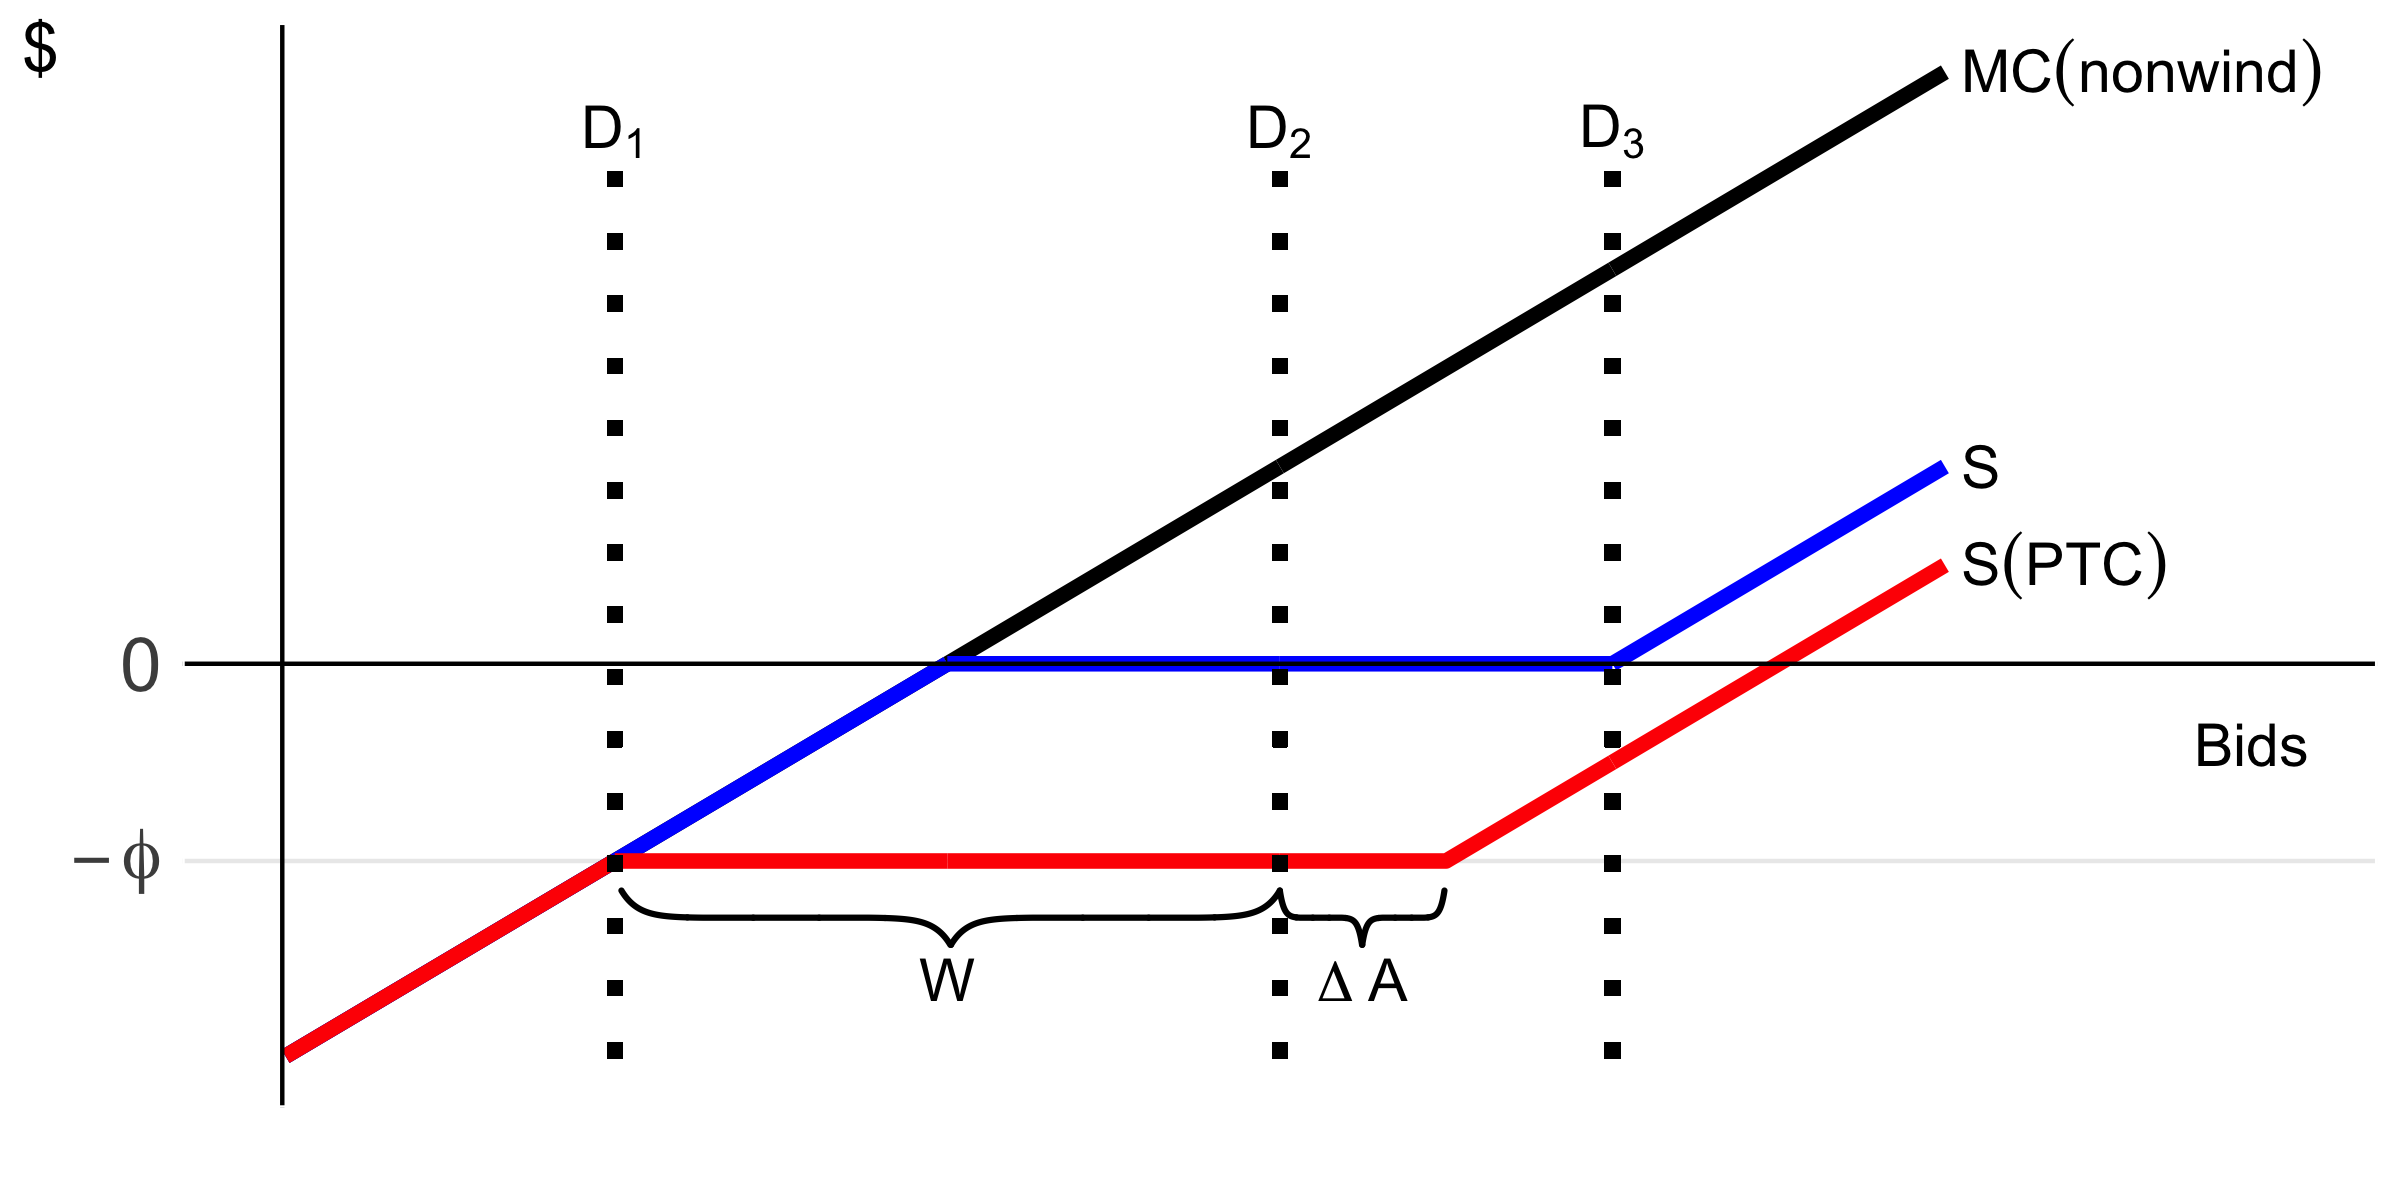
\includegraphics[width=0.85\textwidth]{../output/figures/dispatch.png}
\end{figure}

An output subsidy of $\phi$ per MWh of wind generation moves wind up in the dispatch curve, displacing some previously inframarginal non-wind capacity. This is because wind farms dispatched at a price of $-\phi$ will have net zero private marginal profits after accounting for the subsidy. The output subsidy also increases the availability of wind farms for the reasons discussed above. This boost in available capacity is represented by $\Delta A$ on the graph. The resulting supply curve is \textbf{S(PTC)}. 

Comparing \textbf{S} and \textbf{S(PTC)} shows how, conditional on installed capacity, the net change in wind power generated, and the mechanism behind that change, depend on the level of demand. For very low levels of demand, below $D_1$, there is no difference in wind generation under the two subsidies because no wind is dispatched in either case. For demand between $D_1$ and $D_2$, the output subsidy increases wind generation via the dispatch effect. For demand between $D_2$ and $D_3$, the difference is due to both the dispatch and availability effects. Finally, for levels of demand above $D_3$, any difference in output across the two subsidy types comes entirely from the availability effect.

\section{Data\label{sec:Data}}

In this section, we concisely summarize our data sources and sample restrictions. Additional detail is provided in Appendix~\ref{sec:Data_Appendix}. We compiled data on wind farm characteristics and output from two publicly available Energy Information Administration (EIA) surveys covering all utility-scale wind farms in the United States. The EIA-860 database, which reflects an annual survey of power plants, contains: first date of commercial operation, operator, location, nameplate capacity, number of turbines, predominant turbine model, average annual wind speed,\footnote{We also refer to EIA's average annual wind speed as ``design wind speed'' to distinguish it from wind speed data from 3TIER.} wind quality class,\footnote{Wind quality class takes one of four categories defined by the International Electrotechnical Commission.} regulatory status of the plant, entity type\footnote{The entity types recorded on Form EIA-860 are: cooperative, investor-owned utility, independent power producer, municipally-owned utility, political subdivision, federally-owned utility, state-owned utility, industrial, and commercial. We use this information to restrict our sample as described in the text. We also use it to construct a dummy variable for independent power producer (IPP) that we include in our analysis in order to capture variation in ownership structure conditional on regulatory status, as some non-regulated plants are owned by investor-owned utilities.} of the principle owner, and operation within a regional transmission organization (RTO) or independent system operator (ISO). We combine this annual plant-level information with monthly electricity generation data collected through the Form EIA-923 survey of power plants.

We supplement these EIA data with proprietary data from the American Wind Energy Association (AWEA), 3TIER, and turbine manufacturers. The AWEA database contains additional cross-sectional information on each wind farm, including the wind turbine model and whether projects contract output through long-term power purchase agreements (PPAs) or sell on spot markets. We use the former to corroborate turbine data in the EIA-860 and the latter to construct ``offtake type'' indicator variables which control for potentially differential contracting arrangements across 1603 and PTC recipients in the estimated regression models.

3TIER uses global wind and weather monitor data to interpolate hourly wind speed, wind direction, air pressure, and temperature for the entire continental United States at a spatial resolution of approximately 5 kilometers.\footnote{For more information on how this dataset is constructed, see: \href{http://www.3tier.com/en/support/wind-prospecting-tools/how-was-data-behind-your-prospecting-map-created/}{http://www.3tier.com/en/support/wind-prospecting-tools/how-was-data-behind-your-prospecting-map-created/} (Accessed 2/14/2017).} We combine these high frequency wind data with power curves from turbine manufacturers for each turbine make and model in the EIA data.\footnote{Power curves were primarily obtained from \href{http://www.wind-power-program.com/}{http://www.wind-power-program.com/} (last accessed 2/14/2017), and supplemented with information obtained directly from turbine manufacturer marketing materials (generously provided to us by Joern Huenteler).} Using this information, we compute an ``engineering'' estimate of the potential output for each plant-month that accounts for the site-specific, nonlinear relationship between wind speeds and electricity generation. Further detail on this variable and its construction is provided in Appendix~\ref{Appendix:Potential-capacity-factor}.

The final dataset comes from the U.S. Department of Treasury. The dataset provides information on every large wind project recipient of a 1603 grant, including the amount awarded (equal to 30 percent of eligible investment costs), the date of the award, and the date placed in service.\footnote{The Department of the Treasury distinguished between ``large'' wind projects, which are eligible for the PTC, and ``small'' wind projects, which must have nameplate capacity no greater than 100 kilowatts and are eligible for investment tax credits. All utility-scale wind projects and all wind farms in the data compiled from the EIA fall into the ``large'' wind project category. } We assume that all developers of non-1603 recipient wind farms claimed the PTC based on both guidance provided by staff at the American Wind Energy Association and Internal Revenue Service data. Specifically, we confirmed that no corporation claimed the ITC for PTC-eligible projects (i.e., wind) in 2009, 2010, and 2011 in the annual Internal Revenue Service Estimated Data Line Counts reports for corporation tax returns. We do not have plant-specific tax data on the PTC claims, although we observe all power related data for presumed PTC-claimants through the EIA data described above.

Appendix table~\ref{tab:Summary-Statistics} presents an annual summary of these data for plants entering service between 2002 and 2014.\footnote{There are two potential ways to define online date based on the EIA data. One is the date that the survey respondent reports to EIA that the plant began commercial operation on Form EIA-860; the other is the first date that its generation appears in the EIA-923 production data. Although these by and large coincide, discrepancies can appear due to ``pre-commercial'' plant testing (923 date \textless{} 860 date) or due to the delay with which EIA begins tracking new plants (860 date \textless{} 923 date). This is important because the online date determines 1603 grant eligibility (our instrument). We use the 860 date, as we were told by an EIA expert that this date would be more accurate for our purposes. Nevertheless, IV results are robust to using the 923 date instead. In all specifications, plants with conflicting 923 and 860 dates around the 2009 eligibility cutoff are excluded from the sample.} In our empirical analysis, we restrict attention to plants with owners classified as either independent power producers or investor-owned utilities. Commercial and industrial facilities are excluded, as are plants that are publicly owned (e.g., municipal power plants), as these plants are not eligible for the PTC. We also exclude a small number of plants that appear to have claimed the PTC for some turbines that came online before 2009 and the Section 1603 grant for some turbines that came online in 2009 or later (see Appendix~\ref{sec:Data_Appendix} for further details).

Table~\ref{tab:ttest:ptcvs1603} compares projects placed into service during the 1603 grant eligibility period by subsidy type. Although the overall project sizes are comparable\textemdash both in terms of total size (i.e., nameplate capacity) and turbine size\textemdash 1603 recipients are located in areas with slightly lower average wind speeds, are less likely to operate in a regulated market, and are more likely to contract output through PPAs. Figure~\ref{map:2009to2012} presents a map of plant locations coded by subsidy choice. Although there is considerable spatial overlap in many parts of the U.S., some regions show a clear preference among developers for one subsidy type. Together, these differences are suggestive of selection.

Projects selecting the 1603 grant also have lower potential and realized capacity factors.\footnote{Capacity factors, which effectively measure power plant capacity utilization, are a commonly used metric of operational activity in the electric power sector \citep[see, for example,][]{davis_deregulation_2012}. Additional detail provided in Appendix~\ref{Appendix:Potential-capacity-factor}.} A capacity factor is the ratio of output to the maximum attainable output of a plant if it continuously produces electricity at its nameplate capacity. Here, the \textit{potential} capacity factor is an engineering-based prediction of the capacity factor computed using each plant's wind turbine and wind speed data. The \textit{realized} capacity factor (henceforth simply ``capacity factor'') is constructed using the plant's actual output. Thus, the final row of Table~\ref{tab:ttest:ptcvs1603} shows that 1603 recipients produce less electricity than PTC recipients on average, relative to their total potential output. In the next section, we describe our strategy for identifying the portion of this observed difference in productivity attributable to the subsidy rather than selection.

\begin{table}[h]
\caption{Comparison of 2009-2012 Projects by Policy Choice\label{tab:ttest:ptcvs1603}}
\input{../output/tables/ttest_PTCvs1603.tex}
\footnotesize
Each row contains a two-sample t-test for a difference in means between recipients of the PTC and the Section 1603 grant that came online in 2009-2012 and are in the restricted sample described in Section~\ref{sec:Data}. Regulated, IPP, and PPA are binary variables. Potential Capacity Factor and Capacity Factor are ratios (scaled by 100), both of which are computed using data from 2013 and 2014.
\end{table}

\section{Empirical Strategy and Productivity Results \label{sec:Empirical-Strategy}}

Motivated by the previous discussion of the potential for output subsidies to increase wind farm productivity, we quantify the magnitude of this effect by estimating following regression under several different assumptions and sample restrictions:

\begin{equation}
q_{it}=\delta D_{i}+\beta X_{it}+\nu_{it}\label{eq:second_stage}
\end{equation}
where $q_{it}$ is plant $i$'s capacity factor (in percentage points) in month-year $t$; $X$ is a vector of controls, such as engineering-based potential capacity factor, regulatory regime, presence of a power purchase agreement, and location dummies; and $D$ is an indicator for whether wind farm $i$ took the 1603 grant. The coefficient of interest, $\delta$, reflects the effect of \emph{removing} output subsidies. Given the preceding discussion of two channels through which output subsidies can increase production, we expect $\delta$ to be negative.

Estimating equation~\ref{eq:second_stage} using OLS is problematic due to the fact that wind farms had to opt in to the 1603 program, so $D_{i}$ was chosen. Intuitively, plants that expect to have high output relative to their investment costs will prefer the PTC, while plants with relatively high investment costs per unit of expected output will prefer the Section 1603 grant. Thus, OLS estimates could confound the response to reducing marginal production incentives with the fact that less productive plants are likely to have selected into the 1603 grant program. To address this concern, we employ two complementary empirical approaches to identify the causal effect of the Section 1603 grant on wind farm output: an instrumental variables estimator and a matching estimator.

\subsection{Instrumental Variable Estimation}

Our primary empirical strategy harnesses the natural experiment created by the 1603 grant program by comparing wind farms that came online just before and just after the program went into effect. While the Section 1603 grant was not randomly assigned, its creation came as a plausibly exogenous shock to the industry. We exploit this shock by using a binary indicator for whether the project came online after January 1, 2009 as an instrument for cash grant recipient status. We use this instrument along with wind farms' monthly output data over 2010-2014 to estimate equation~\ref{eq:second_stage} via two-stage least squares. This IV approach is similar to a fuzzy regression discontinuity design with time as the running variable, which we implement as a sensitivity analysis in Appendix Table~\ref{tab:rdd_cf_linear}.

Identification and interpretation of $\delta$ relies on two key assumptions: (1) that ineligible firms cannot manipulate the date they came online to receive the subsidy, and (2) that the instrument (subsidy eligibility) only affects outcomes through its effect on the endogenous variable (subsidy choice).\footnote{Identification and interpretation as a local average treatment effect also relies on three other restrictions/assumptions. First, we know from the data that the first stage is non-zero. Second, the monotonicity assumption holds by virtue of the policy environment: firms cannot ``defy'' treatment assignment because the 1603 grant is only available from the Federal government. Finally, we assume homogeneous treatment effects.} The first assumption is supported by institutional details. Wind farms could not strategically adjust when they came online in anticipation of the policy, as the policy had not even been proposed until after the January 1, 2009 eligibility date (see Section~\ref{subsec:RenewablePolicies}). 

To assuage concerns about the exclusion restriction, our main IV specification uses a bandwidth of one year on either side of the start date of the policy, relying only on a comparison of projects that came online in 2008 and 2009. This has two main advantages. First, long-run trends in wind turbine technology and electricity markets are less likely to influence our results. For example, $\input{../output/estimates/stat_pct_same_turbines.tex}$ percent of the new projects in our 2008-2009 sample use turbine models that were used in both years. Second, projects that came online in early 2009 were planned and began construction in 2008 (or earlier), which implies that these plants were originally designed for the PTC \citep{bolinger_preliminary_2010}. This helps mitigate concern that 1603 grant recipients are fundamentally different, as may be the case in later periods. 

Table~\ref{tab:ttest_RD_sample_pre} compares projects coming online in 2008 with those coming online in 2009 using two-sample t-tests. In contrast to the comparison of PTC and 1603 plants over the full life of the policy (Table~\ref{tab:ttest:ptcvs1603}), the two groups in Table~\ref{tab:ttest_RD_sample_pre} are statistically indistinguishable in terms of several pre-treatment characteristics including turbine size, wind speed, regulatory status, and whether a wind farm has entered into a PPA. Similarly, despite small differences in subsidy preference across regions in 2009, Figure~\ref{map:2008to2009} shows that both subsidy types have strong spatial overlap with PTC plants that came online in 2008, which is the relevant comparison in this analysis. Nonetheless, capacity and the probability of being an independent power producer are statistically different in Table~\ref{tab:ttest_RD_sample_pre} across these two years. To account for this, we condition on these variables in our regressions. 

\begin{table}[H]
\caption{Projects Entering One Year Before and After the Policy\label{tab:ttest_RD_sample_pre}}
\input{../output/tables/ttest_2008vs2009.tex}
\footnotesize
Each row contains a two-sample t-test for a difference in means between wind farms that came online in 2008 and in 2009 and that are in the restricted sample described in Section~\ref{sec:Data}. Regulated, IPP, and PPA are binary variables. Potential Capacity Factor and Capacity Factor are ratios (scaled by 100), both of which are computed using data from 2013 and 2014.
\end{table}

Most importantly, the plants in these two years have remarkably similar engineering-based potential capacity factors. However, our outcome variable, \textit{realized} capacity factor, is lower (and statistically distinguishable) for projects coming online in 2009 than for projects coming online in 2008. This difference in observed productivity, despite the lack of difference in potential productivity, provides an (unscaled) preview of the main IV results. 

\subsubsection*{Results \label{sec:results:rd}}

Table~\ref{tab:rdd_cf} reports the instrumental variable results. The sample is restricted to a balanced panel of monthly generation from 2010 to 2014 at wind farms that came online in 2008 or 2009. The dependent variable in each regression is the capacity factor in percentage points.

\begin{table}[h]
\caption{Instrumental Variables Estimates \label{tab:rdd_cf}}
\begin{center} {\footnotesize{}\input{../output/tables/rdd_regressions_cf.tex}} \end{center}
\footnotesize
The dependent variable is the capacity factor in percentage points. Data include a balanced panel of monthly observations from 2010 to 2014 for all wind farms. All models contain year-month dummies. Standard errors clustered by wind farm reported in parentheses.
\end{table}

The primary coefficient of interest ($\delta$) appears in the first row of the table, labeled 1603 Grant. The first three columns present OLS estimates of equation~\ref{eq:second_stage}. Column 1 includes only time (month-year) dummies. The interpretation is that plants receiving output subsidies operated at 5 percentage points lower capacity factor compared to PTC recipients coming online between 2008 and 2009. Column 2 adds controls for plant size and monthly wind quality, as well as dummies for whether the plant is regulated, whether it is owned by an independent power producer, and presence of a power purchase agreement.\footnote{Unless otherwise noted, the same controls appear in every model throughout the paper. Additional discussion of the potential capacity factor and wind speed variables is provided in Appendix~\ref{Appendix:Potential-capacity-factor}.} Consistent with the descriptive evidence above, 1603 and PTC plants differ on observable dimensions, and controlling for these differences reduces the estimated productivity gap. Column 3 adds state fixed effects to account for other unobserved differences in markets and renewable policies across states, which attenuates the relationship further.

Columns 4-6 present IV estimates using the same covariates, instrumenting for 1603 receipt with an indicator for whether the wind farm was eligible for the 1603 program. Conditioning only on month of sample, 1603 plants are 3.7 percentage points less productive than their PTC counterparts. This difference is considerably smaller than the OLS estimate in column 1. Adding controls results in a modestly lower estimated 1603 effect of 2.9 percentage points, and is our preferred specification. Column 6 adds state fixed effects, which effectively discards 25 percent of the sample for which there is no within-state subsidy variation. The estimate splits the difference between the previous two, leaving a 3.2 percentage point gap in productivity across plants choosing the two subsidy types. Our preferred estimate of \input{../output/estimates/stat_rd_estimate.tex}implies that 1603 grant recipients would have produced roughly \input{../output/estimates/stat_rd_estimate_pct.tex}percent more power had they claimed the PTC.\footnote{This 10 percent reduction is computed by dividing the estimated \input{../output/estimates/stat_rd_estimate.tex}percentage point reduction in capacity factor by the average capacity factor for all 1603 grant recipients of \input{../output/estimates/stat_avg_cf_1603.tex}percentage points.} To provide context for the magnitude of this estimate, note that it is in line with industry claims for how post-construction wind farm optimization services could increase output (see discussion in Section~\ref{sec: Background}). The marginal incentive of the PTC is quite substantial during this time period, providing a premium of roughly 40 percent over the average price of power sold by wind farms to the grid. As such, the estimate in column 5 implies a supply elasticity of around 0.25. 

\subsubsection*{Robustness Analysis}

We assess the sensitivity of our results to the assumed sample bandwidth. The primary motivation for doing this is concern about violations of the exclusion restriction. Since our instrument is based on time, we are concerned that it will pick up other factors that impact wind farm productivity independent of the policy. Furthermore, although we believe it is highly unlikely that wind farm developers could have made significant changes to projects that began operations in 2009 after first learning about the policy, that possibility becomes more remote as we shorten the sample around the policy introduction. Of course, smaller bandwidths generate smaller samples, lessening the statistical precision of our estimates. Figure~\ref{fig:CFbandwidths} presents coefficients from the preferred specification in column 5 in graphical form using alternative bandwidths ranging from three months to 24 months on each side of the policy change. Although the confidence intervals are large for the very small bandwidths, the results are consistent and reinforce our baseline findings: all specifications suggest receipt of the 1603 grant leads firms to produce less electricity than they would have if they had received the PTC. Moreover, the fact that the point estimates remain remarkably stable between nine and 24 months assuages concerns that the results are driven mainly by time trends.\footnote{We also estimate models that allow for the possibility of trends within the 2008-2009 time period in technology, site quality, and other factors that have persistent effects on output. Table~\ref{tab:rdd_cf_linear} presents results from a parametric fuzzy regression discontinuity model that includes piecewise linear trends. Unfortunately, given the small sample size, these results are quite noisy. In models 4 and 5, the point estimates are larger in magnitude than the IV estimates, while in model 6 the results are smaller and not statistically distinguishable from either the IV estimates or zero. The variability in these estimates may be the result of weak instruments, as they have relatively small first-stage F-statistics.}

\begin{figure}[H]
\caption{IV Estimates using Alternative Bandwidths \label{fig:CFbandwidths}}
\vspace{-15pt}
\begin{center}
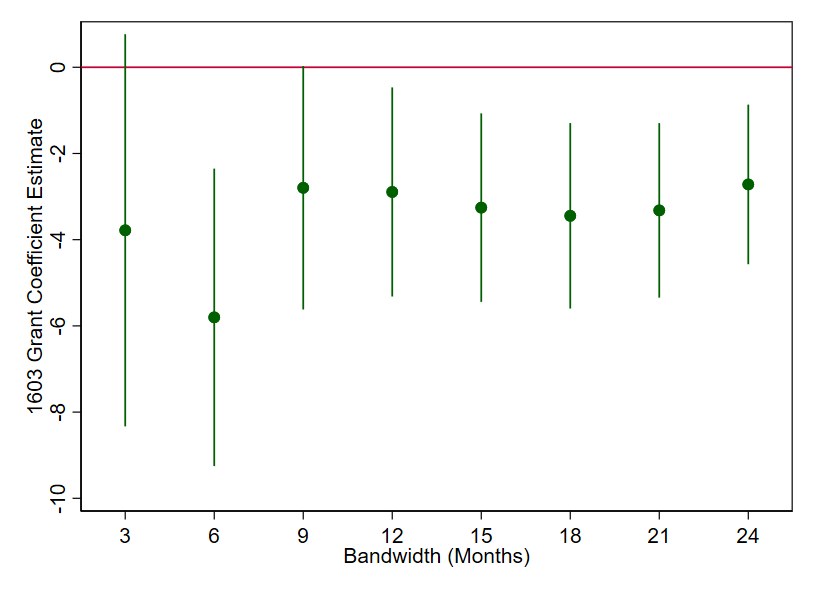
\includegraphics[width=0.75\textwidth]{../output/figures/fuzzyRDD_capfactor_bandwidths_nostateFEs.png}
\end{center}
\vspace{-15pt}
\footnotesize
Coefficient estimates from 2SLS regressions of capacity factor on a binary indicator for 1603 grant receipt, instrumented with a binary indicator for grant eligibility. Regressions also include year-month dummies, controls for plant size and wind quality, as well as dummies for whether the plant is regulated, is owned by an IPP, and has a PPA. Data are a panel of monthly observations from 2010 to 2014. Each point corresponds to a sample defined by its bandwidth around January 1, 2009, so that the leftmost model includes plants that came online between October 2008 and March 2009, and the rightmost model includes plants that came online between January 2007 and December 2010. A bandwidth of 12 months corresponds to column 5 of Table \ref{tab:rdd_cf}. Spikes denote 95\% confidence intervals based on standard errors clustered by wind farm.
\end{figure}


\subsection{Matched Differencing \label{subsec:Matching}}

Our second empirical strategy uses a combination of matching and differencing to infer counterfactual outcomes for 1603 grant recipients. Assume the unobserved component of production takes the form $\nu_{it}=A_{i}+\epsilon_{it}$, where $A_{i}$ denotes the unobserved quality of wind farm $i$. Selection in our context would manifest itself as a correlation between $A_{i}$ and $D_{i}$. Conditioning on $A_{i}$ would eliminate this bias, as $E[q_{it}|X_{it},A_{i},D_{i}=1]$=$E[q_{it}|X_{it},A_{i},D_{i}=0]+\delta$. Under the assumption that $A_{i}$ is time-invariant, the use of plant fixed effects with panel data would remove this bias.

Since subsidies are irreversibly chosen at the commencement of operations, we do not observe subsidy variation within a plant, and thus cannot include plant fixed effects. Instead, we adopt the additional assumption that unobserved heterogeneity takes the following form, $A_{i}=g(X_{i})+\gamma Post_{i}$, where $g()$ is an unknown function of observable wind farm characteristics, and $\gamma$ is a wind farm vintage fixed effect for plants entering post-ARRA. Although $g()$ is unknown, including a dummy variable for each unique combination of characteristics $X_{i}$ would fit any $g()$. The difference in productivity between two wind farms with the same characteristics that entered in different policy periods would then simply be $\gamma$.

While we cannot fit $g()$ exactly given that $X_{i}$ contains continuous covariates and our sample is finite, we approximate $g()$ by matching wind farms with similar characteristics across different vintages. We divide our sample into two groups corresponding to two policy regimes: wind farms that entered between 2005 and 2008 (``pre'' plants), when there was no subsidy choice, and wind farms that entered between 2009 and 2012 (``post'' plants), which could choose either the PTC or the 1603 grant. We then match pre and post wind farms on observable characteristics using coarsened exact matching.\footnote{\citet{iacus_causal_2012} outline the algorithm and derive its statistical properties. More information and implementation packages can be found at \href{http://gking.harvard.edu/cem}{http://gking.harvard.edu/cem}.} Let $g$ index a group of pre and post plants that are matched together. Equation~\ref{eq:second_stage} becomes, 

\begin{equation}
q_{it}=\delta D_{i}+\beta X_{it}+A_{g}+\gamma Post_{i}+\epsilon_{it}\label{eq:mdd} ,
\end{equation}
where $Post_{i}$ is an indicator for whether a plant came online after the 1603 program was introduced. Intuitively, the estimator takes the average difference between 1603 recipients and their pre-period matched counterparts, and subtracts the difference between post-period PTC plants and matched pre-plants within their group. To see this, let $D_{g}$ indicate the \emph{observed} subsidy choice of the post-period plants in group $g$. Then
\[
E[q_{it}|D_{g}=0,Post_{i}=1]-E[q_{it}|D_{g}=0,Post_{i}=0]=\gamma
\]
\[
E[q_{it}|D_{g}=1,Post_{i}=1]-E[q_{it}|D_{g}=1,Post_{i}=0]=\gamma+\delta
\]
In practice, we replace $\gamma$ with fixed effects for cohort (i.e., the first year each wind farm generated electricity), and allow group-level unobservables to vary by time.

Matching requires us to drop plants that do not lie within the common support of pre and post period entrants on key observable dimensions. Within the set of plants that remain, identification requires assuming there are no unobservables that affect both production changes across pre and post plants and subsidy choice (i.e., unconfoundedness). We also assume the covariates used for matching are unaffected by the availability of the 1603 grant. While we cannot directly assess this assumption, the long development timeline of wind farms reduces concern over any large responses on this dimension. Moreover, the IV analysis addresses precisely this concern.

The primary concern with the IV estimator is that the instrument, time, may be picking up other trending factors that affect productivity. Our matching estimator relaxes this by allowing unobservable dimensions of wind farm entry cohorts to evolve over time. The key assumption is parallel trends in these unobservable factors across the types of plants that choose each subsidy in the post period. 

\subsubsection*{Results \label{sec:results:matching}}

We match exactly on several categorical variables (geography, wind quality class, regulatory status, and entity type) and two coarsened continuous variables (capacity and design wind speed).\footnote{In this analysis, we match on two wind quality measures collected by the EIA, design wind speed and wind class. An alternative would be to match on the realized potential capacity factor, which we construct and use as a control at the month level, averaged over the sample. We prefer the EIA measures because they are directly reported to the EIA, and likely more accurate in the cross section. These two measures are also widely used in the industry, with wind class (a categorization of site wind variability) used as a critical determinant of which turbines can safely be placed at a location. Moreover, the conceptual exercise here is to match similar \textit{sites} in the pre and post policy period, while the potential capacity factor combines both site and time-varying technology changes. With that said, the results are qualitatively similar when we match on potential capacity factor instead. These are presented in appendix Table~\ref{tab:matching_group_ptnlcf}.} This procedure selects all pre-period wind farms within the same coarsened cell in the covariate space as each post-period wind farm.

Table~\ref{tab:matching_balance} compares pre- and post-period entrants after using coarsened exact matching with state as the geography. Of the 465 wind farms in our sample entering between 2005 and 2012, 204 lie within the common support of these variables across the two policy periods.\footnote{The number of post-period matches is higher than pre-period matches because more post-period plants fall within the same coarsened cell than do pre-period plants.} The number of post-period 1603 matches is about double the number of PTC matches, which is in line with their underlying population probabilities. T-tests confirm that this restricted sample is in fact balanced across the two time periods on the matched dimensions. In particular, the two dimensions that were imbalanced in the IV sample, capacity and IPP status, are now statistically equivalent across the pre and post periods in this sample by construction. 

\begin{table}[h]
\caption{Matching Balance \label{tab:matching_balance}}
\input{../output/tables/matching_balance.tex}
\footnotesize
Each row contains a two-sample t-test for a difference in means between wind farms that came online before versus after January 1, 2009 that meet sample restrictions described in Section~\ref{sec:Data} and are selected using coarsened exact matching. See text for more details on the matching procedure. Regulated and IPP are identical across samples by construction. Regulated, IPP, and PPA are binary variables. Potential Capacity Factor and Capacity Factor are ratios (scaled by 100), both of which are computed using data from 2013 and 2014.
\end{table}

Table~\ref{tab:matching_group} reports the results from regressions estimated through variations of this matching strategy with an unbalanced panel of monthly wind farm production data from 2009 to 2014. As before, the dependent variable in each regression is the capacity factor measured in percentage points. All models include the same controls as our preferred IV regressions as well as dummies for cohort (i.e., the first year each wind farm generated electricity). Column 1 presents estimates from estimating OLS on the full sample including all 465 wind farms entering during the pre- or post-period. Column 2 restricts the sample to plants matched across periods. Column 3 includes matched group fixed effects. Column 4 interacts those group fixed effects with year of sample, allowing for unobserved factors that affect specific groups and vary over time. Column 5 includes group-year-month fixed effects. 

Simply restricting the sample to observably similar plants across periods increases the estimated impact of the 1603 grant from 2.9 to 4 percentage points. This suggests that there are low productivity PTC plants and/or high productivity 1603 plants that do not lie in the common support across periods. Allowing for increasingly time-varying group level unobservables has remarkably little effect on the estimates. The estimated productivity reduction in column 4 of \input{../output/estimates/stat_match_estimate.tex}percentage points (\input{../output/estimates/stat_match_estimate_pct.tex}percent) is similar to our preferred IV estimate, despite relying on different identifying assumptions.

\begin{table}[h]
\begin{center}
\caption{Matching Estimates \label{tab:matching_group}}
\input{../output/tables/exact_match_state.tex}
\end{center}
\footnotesize
The matched sample was constructed using coarsened exact matching on state, wind quality class, regulatory status, entity type, capacity, and design wind speed. All models include the controls listed in the IV models in Table~\ref{tab:rdd_cf}: log capacity, potential capacity factor, and wind speed variance, as well as dummies for whether the plant is regulated, whether it is an IPP, the presence of a PPA, and month of sample. All models also include cohort dummies. Models are estimated using an unbalanced panel of monthly wind farm production data from 2009 to 2014. Standard errors, clustered at the plant level, are reported in parentheses.
\end{table}

\subsubsection*{Robustness Analysis}

The most restrictive matching criteria in the previous exercise is the requirement that pre and post plants be in the same state. In order to explore the impact of this assumption, and to incorporate more plants into the analysis, we re-estimate the model from column 4 under different geographic restrictions (Table~\ref{tab:matching_table_cf}). As above, all models use coarsened exact matching on geography, wind quality class, regulatory status, entity type, capacity, and design wind speed. In addition, column 1 matches on NERC region as well as an indicator for whether the plant is in an ISO. Column 2 matches on the specific ISO a plant participates in, and column 3 matches on both NERC region and ISO. Finally, column 4 matches on state, repeating column 4 from the previous table. In addition to controls, month of sample dummies, and matched group-year dummies, each of the first three models also include state fixed effects to account for differences in state-level renewable policies. As in the previous table, the results increase slightly as increasing restrictions are placed on the matching procedure. However, we cannot statistically distinguish among the coefficient estimates.

\begin{table}[H]
\begin{center}
\caption{Sensitivity of Matching Estimates to Geographic Restrictions \label{tab:matching_table_cf}}
\input{../output/tables/exact_match_wide_table.tex}
\end{center}
\footnotesize
Matched samples constructed using coarsened exact matching on geographies listed in the table, wind quality class, regulatory status, entity type, capacity, and design wind speed. All models include the controls listed in the IV models in Table~\ref{tab:rdd_cf}: log capacity, potential capacity factor, and wind speed variance, as well as dummies for whether the plant is regulated, whether it is an IPP, the presence of a PPA, and month of sample. All models also include cohort dummies, matched group-year fixed effects, and state fixed effects. Models are estimated using an unbalanced panel of monthly wind farm production data from 2009 to 2014. Standard errors, clustered at the plant level, are reported in parentheses.
\end{table}

\section{Discussion \label{sec:Discussion}}


\subsection{Mechanism and Interpretation \label{sec:Mechanism}}

We estimate that selecting the 1603 grant, an investment subsidy, caused wind farms to produce about \input{../output/estimates/stat_rd_estimate_pct.tex}percent less output than they would have under the PTC, an output subsidy. The discussion in Section \ref{subsec:outputModel} presents two mechanisms through which this might occur: a ``dispatch'' effect, causing wind to displace some previously inframarginal generation at low demand levels, and an ``availability'' effect, causing wind to displace marginal generation at all other demand levels. How much of the estimated difference in output across PTC and 1603 plants can be attributed to each channel? Since we only observe monthly plant production, we cannot answer this question directly.\footnote{In Appendix~\ref{Appendix:NegativePrices}, we compile statistics on the frequency of negative prices, which are an indictor that wind might be near the margin. While the frequency varies considerably across time and space, monthly shares exceeding our estimated productivity effect are not uncommon. This suggests that it's possible that increased dispatch alone could explain the output effect of the 1603 grant. We do not have any statistics to similarly judge the plausible magnitude of the availability affect. However, many consulting companies tout wind farm services which promise increases in productivity of this magnitude. For example, General Electric offers a product called ``PowerUp'', which it describes as ``a customized suite of software and hardware-enabled technologies created to increase a wind farm's output by up to 10\%, taking into account environmental conditions.'' Source: \href{https://www.gerenewableenergy.com/wind-energy/turbine-services/platform-upgrades}{General Electric website} (accessed 1/29/2018).}

Does it matter how much of the estimated output increase comes from dispatch versus availability? While this paper is primarily focused on cost-effectiveness, the two mechanisms have different efficiency implications. An output subsidy that moves wind up in the dispatch order can generate social benefits by reducing externalities from plants that were previously inframarginal to wind during low demand hours. However, this also generates social costs by raising the (private) production cost of electricity during these hours. The net effect depends on whether marginal damages are larger than the production cost differences. In contrast, the availability effect displaces production from plants with higher private production costs than wind. This generates benefits equal to the avoided social costs from these displaced units, including both electricity production cost savings and external damages avoided.\footnote{Increasing availability may involve fixed costs, which we omit here for ease of exposition. In the back of the envelope calculations below, we approximate these fixed costs by assuming that the marginal gains in availability are linear in these costs.}

Figure \ref{fig:mechanism_welfare} presents a graphical representation of these forces, based on the illustrative dispatch curve in Figure \ref{fig:dispatch}. The top row presents the social marginal cost of each unit of generation, ordered by their subsidy-inclusive private marginal costs, with and without the PTC subsidy of $\phi$ to wind generators. For comparison, the dashed line decomposes the PTC line into a case where the PTC affects dispatch but has no effect on availability. Under the standard assumption that electricity demand in any hour is perfectly inelastic, the net benefits of the PTC, relative to no PTC, can be computed as the integral of the difference between the PTC and No PTC cost curves in the corresponding top panel. The bottom panel presents these net benefits at every level of demand.

\begin{figure}[h] 
\begin{center}
\caption{Mechanism and Net Benefits \label{fig:mechanism_welfare}}
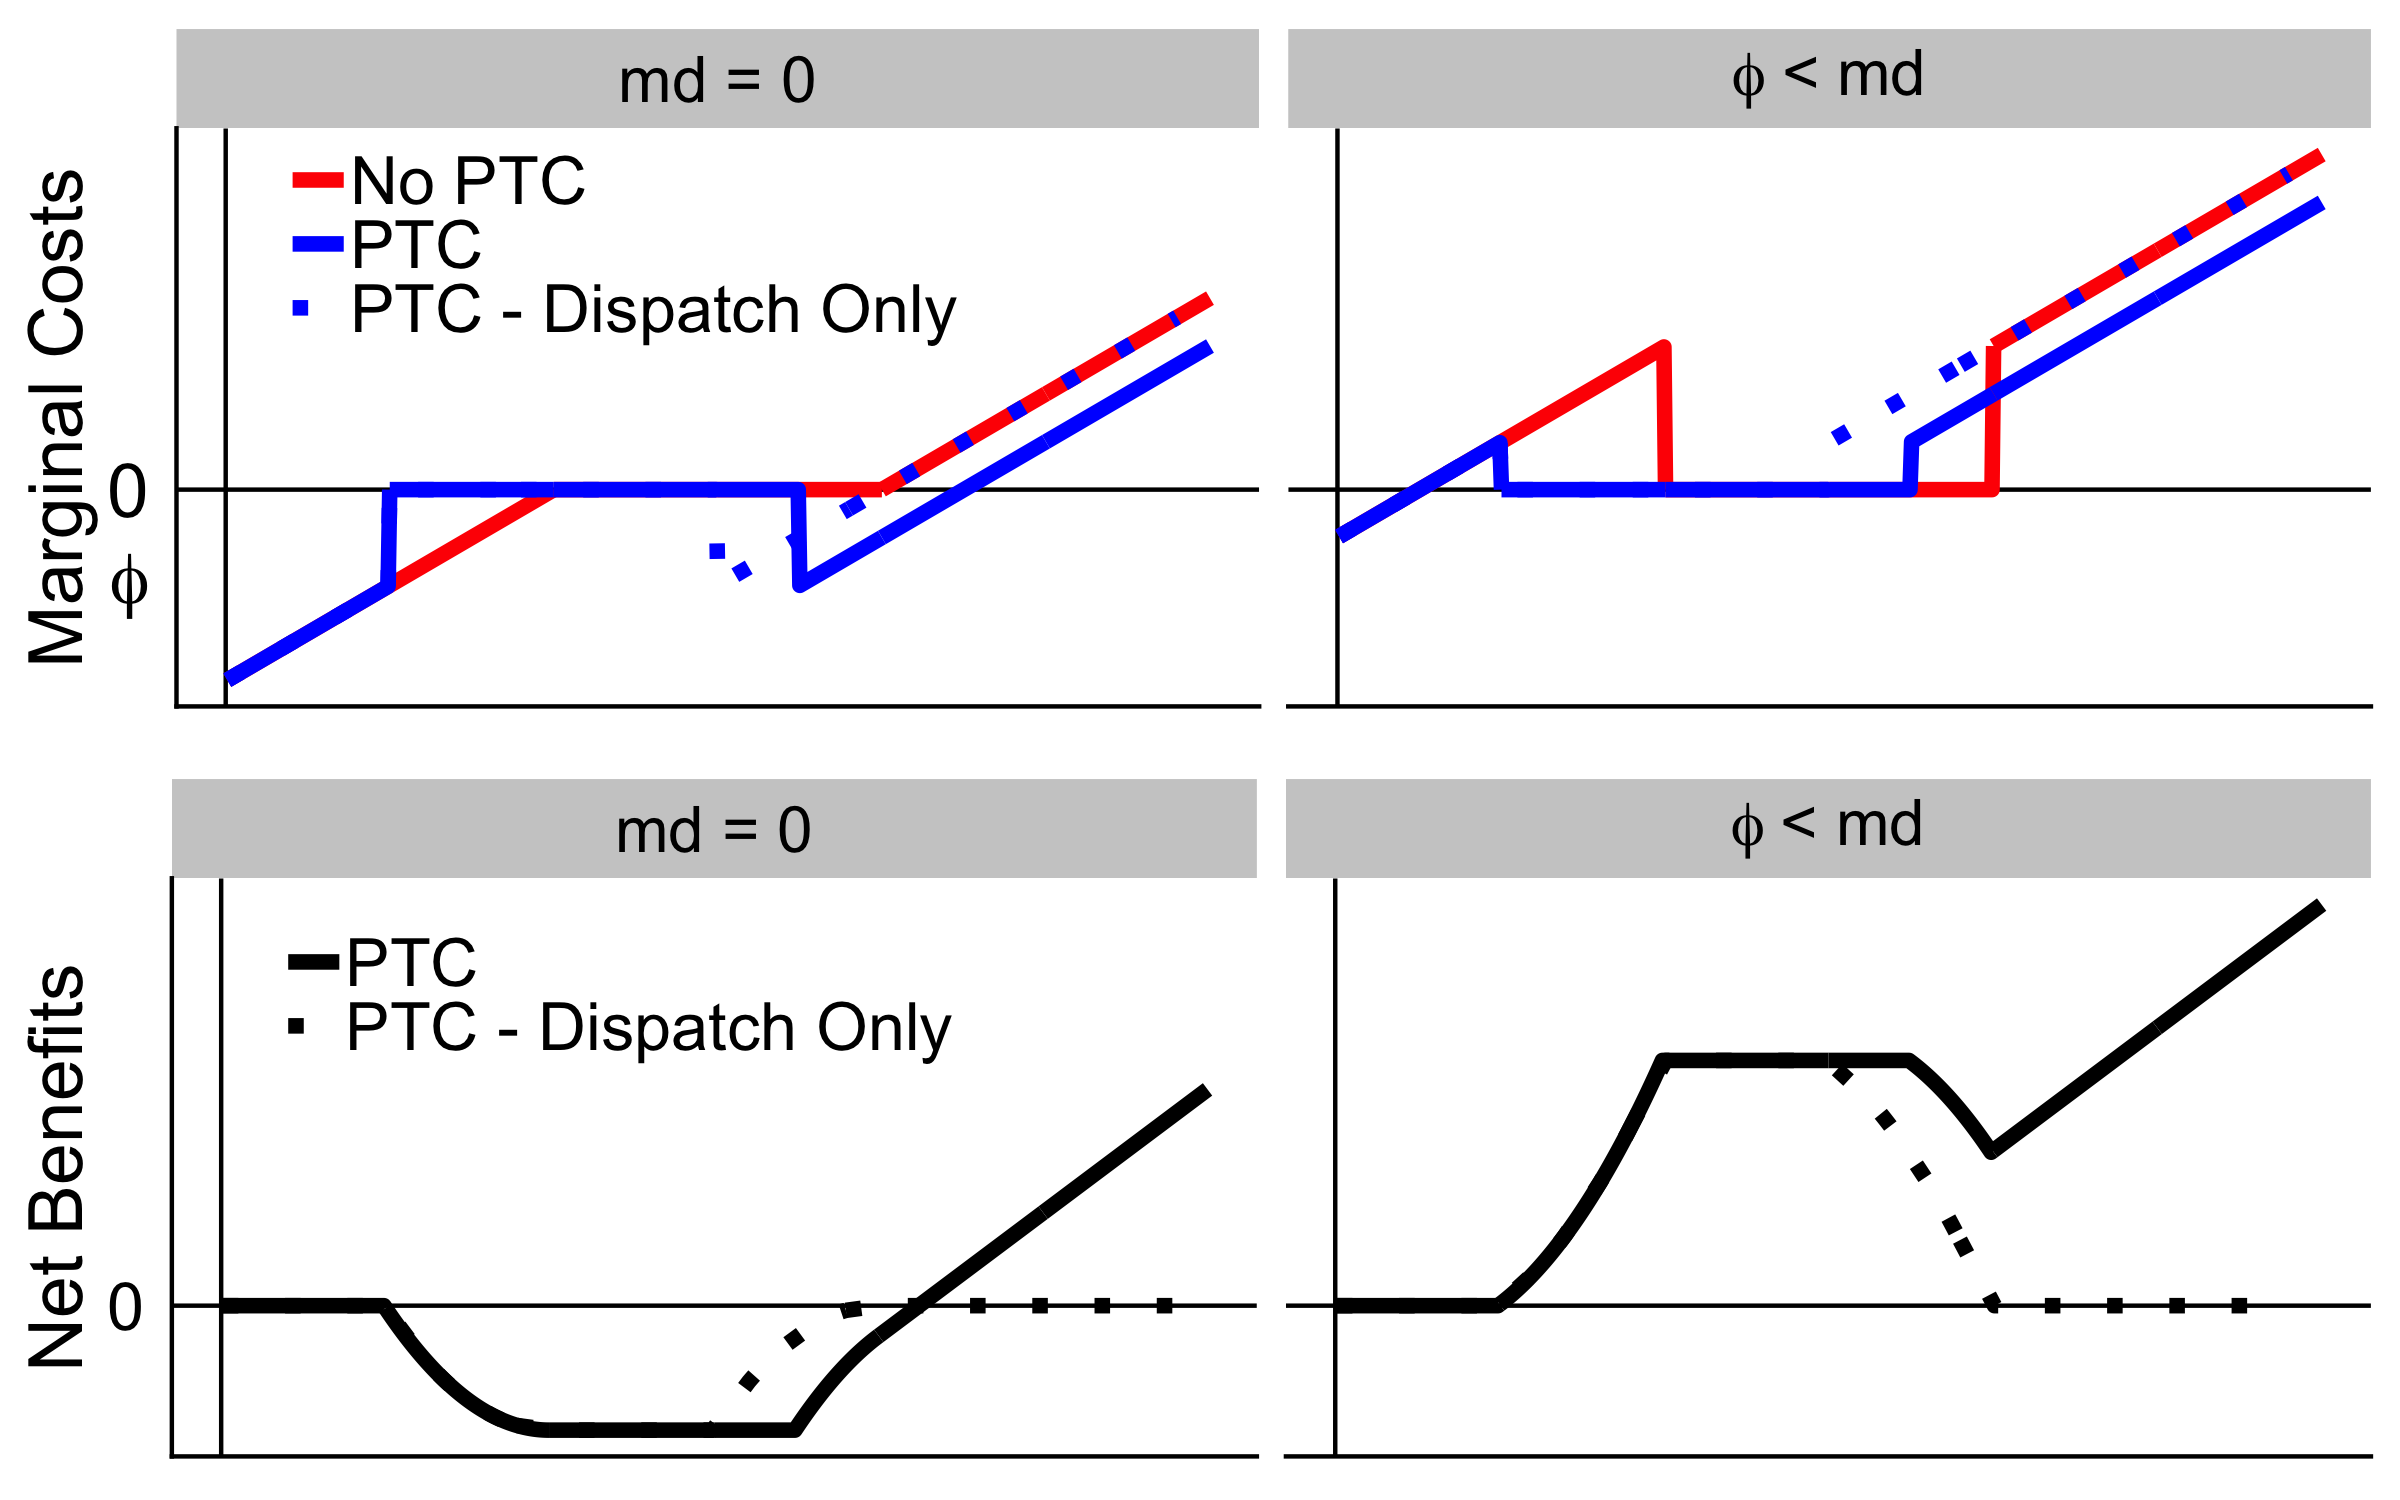
\includegraphics[width=0.85\linewidth]{../output/figures/net_benefits.png}
\end{center}
\end{figure}

The left column of Figure \ref{fig:mechanism_welfare} presents the case where there are no external marginal damages ($md$) associated with non-wind generation (for example, if wind displaces nuclear or hydro). Given that there are no unpriced externalities, the PTC generates welfare losses whenever wind is dispatched and cheaper resources are not. If the PTC increases availability, the net benefits are positive and increasing at high demand levels, because additional wind power displaces marginal plants with high production costs. The right column presents the opposite extreme, where the marginal damages from non-wind generation are larger than the subsidy.\footnote{If wind displaces coal-based power, then the avoided marginal damages from climate change alone would be about \$50/MWh -- double the PTC \citep{iawg_2016}.} If the PTC affects dispatch but not availability, any net benefits from the PTC come entirely during low demand hours. If the PTC also increases availability, net benefits continue to rise at high demand levels, always at a higher level than the $md=0$ case. Intermediate cases where $0 \le md \le \phi$ generate net benefits which lie between these extremes.
% Avoided marginal damages of \$50 per MWh from coal is based on an SCC of $50/metric ton and emissions rate of 2.21 pounds per kWh

Several recent papers provide empirical estimates of marginal damages which suggest our second extreme case -- $\phi < md$  -- holds on average for most regions and time periods across the United States. For example, \citet{holland_are_2016} estimate average marginal damages and find that they are higher than the PTC in most regions and at almost all hours of the day (see appendix Figure \ref{fig:md_np_hmmy}). \citet{fell_emissions_nodate} focus on the environmental benefits of wind electricity and find that annual average marginal damages avoided in MISO and ERCOT are higher than the PTC every hour of the day. As the preceding discussion makes clear, if the entirety of our estimated output effect comes from the dispatch effect, then net benefits depend critically on marginal emission rates during very low demand periods. \citet{callaway_location_2018} estimate the marginal operating emission rates (MOERs) for six large ISOs. In Appendix~\ref{Appendix:NegativePrices} we show that these MOERs are generally highest during the hours of the day and seasons when demand is lowest. The most relevant empirical evidence comes from an econometric study of the marginal emissions impacts of wind power at different levels of demand in Texas, which, conveniently, is also the modal state in our sample. \citet{novan_valuing_2015} finds the marginal external benefits from wind are actually \emph{highest} during periods of low demand because they are most likely to offset non-wind generators that impose large external costs. Based on this evidence, we conclude that the increased wind output generated by the PTC likely increases net benefits \emph{on average} regardless of the mechanism. 

\subsection{Extensive Margin \label{subsec:Extensive}}

So far, we have focused on estimating how much more output 1603 recipients would have produced had they received the PTC, conditional on operating. In this section we consider whether the 1603 program had any effect on the number of plants we observe operating in the first place. This is important because, while our IV and matching estimators address concerns about selection \textit{between} subsidies, both strategies leverage the fact that plants that entered before 2009 did not have access to the 1603 program. If the 1603 grant encouraged more entry, and if these marginal plants were (unobservably) less productive, then extensive margin selection may confound our estimate of the intensive margin response to output subsidies. 

The abrupt introduction of the 1603 program, combined with its short duration relative to project lead times, make it highly unlikely that new wind projects would be conceived entirely in response to the output subsidy. However, at any given point in time, there are many potential projects in various stages of planning, some of which will never come to fruition, and the 1603 grant may have screened in a higher share of these potential projects than in previous years. To assess this, we look for evidence of a change in plant cancellations using the EIA's annual proposed plants list. Figure~\ref{fig:proposed_completed_on_time} presents the share of plants that are completed within one year of their original expected completion year, plotted by expected completion year. The policy period, 2009-2012, is shaded. The completion rates look very similar during the policy period and the years preceding it, and, importantly, the share of plants that are completed does not appear to increase in response to the investment subsidy.\footnote{We also graph the share of plants that are \textit{ever} completed by year of initial proposal in Appendix Figure~\ref{fig:proposed_ever_completed}. Completion rates remain similar before and during the policy period under this alternative metric. This graph also shows that the large drop in on-time completions in 2013 in Figure~\ref{fig:proposed_completed_on_time} indicates delay, not termination, of these post 1603 projects. When Congress extended the PTC for 2013, it made a major change to the eligibility for the tax credit: a wind farm had to begun construction in 2013 to be eligible for the tax credit for its first ten years of generation, in lieu of the previous requirement that a wind farm had to be placed into service.} It thus appears unlikely that productivity estimates will be confounded by low productivity plants being differentially screened in during the policy period. 

\begin{figure}[h]
\caption{Share of Plants Completed on Time, Plotted by Year of Initial Expected Completion\label{fig:proposed_completed_on_time}}
\vspace{-15pt}
\begin{center}
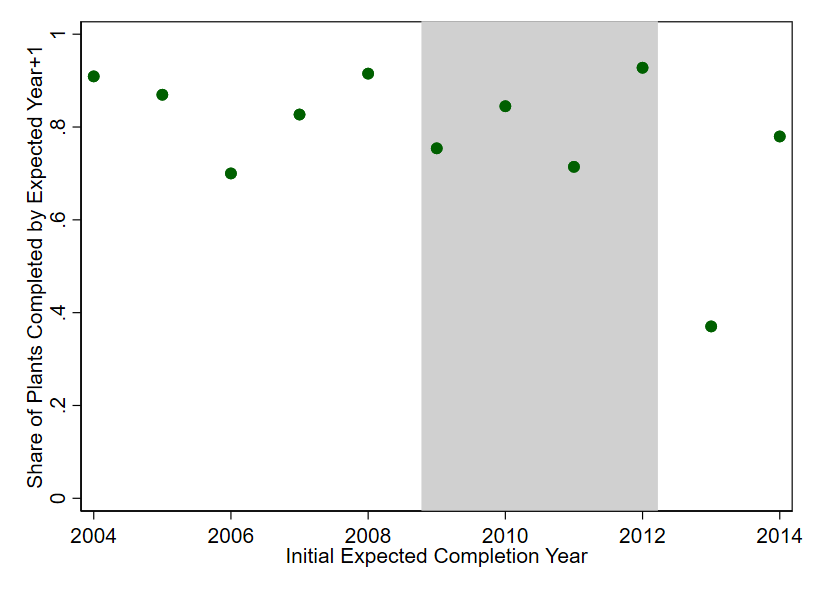
\includegraphics[width=0.75\linewidth]{../output/figures/proposal_data_completed_on_time.png}
\end{center}
\vspace{-15pt}
\footnotesize
The initial expected completion year is the year the generator was first scheduled to start operation. Completion is determined based on whether each plant entered into the EIA-860 operable data. Plots are based on the subset of plants that last appeared in the EIA-860 proposed data prior to 2016. Shading indicates the years during which new plants were eligible for the 1603 grant (2009 to 2012).
\end{figure}

We now consider whether the rate at which projects were completed from 2009 to 2012 would have been \emph{even lower} than previous years absent the 1603 grant program. This program was created in response to the concern that many projects already under development in late 2008 could be rendered unprofitable under the PTC by the widespread financial collapse, as discussed in Section \ref{subsec:RenewablePolicies}. Therefore, while we show that 1603-claiming plants produce less output than they would have under the PTC, we must weigh these inframarginal output losses against any extensive margin gains to compute the net aggregate effect of the program on wind output. Unfortunately, we are unable to estimate the extensive margin effect as rigorously as the intensive margin effect due to the small number of plants entering each period and the time series nature of the policy variation. In lieu of a formal entry model or tests for a time-series break, we instead perform a simple accounting calculation to identify ``marginal'' plants  -- i.e., power plants claiming the 1603 grant that appear profitable under the investment subsidy but not the PTC.\footnote{We describe this calculation briefly here and provide additional details in Appendix~\ref{Appendix:Profitability-calculation-detail}.}

For each 1603 recipient, we construct an estimate of discounted lifetime profits under the program:
\begin{equation}
\pi_i^{1603}=\sum_{t=1}^{t=25} \left(\frac{p_{it}}{(1+r)^{t}}\right) Q_{it} - \frac{c_{it}}{(1+r)^{t}} -(1-s)F_i\label{eq:pi1603} \quad
\end{equation}
Plant-specific output prices ($p_{it}$) are obtained from resale revenues reported on EIA Form 923 and power purchase agreements from AWEA and Bloomberg New Energy Finance (BNEF). We also include in $p_{it}$ estimated marginal revenue from the sale of RECs under state-level renewable portfolio standards using data from Marex Spectron and Lawrence Berkeley National Laboratory. Plants are assumed to remain in service for 25 years ($t$), and right censored prices and quantities are imputed with the observed (real) averages for each plant. Annual net revenue is obtained by subtracting operations and maintenance costs ($c_{it}$) of \$29/kW/year \citep{wiser_2018_2019}, and these flows are discounted at an assumed five percent real interest rate ($r$). Fixed investment costs ($F_i$) are obtained by dividing the observed 1603 grant award amount from Treasury by the fraction of investment costs covered by the program ($s=0.3$).

To compute ``counterfactual'' profits under the PTC we make two modifications to the discounted profit function:
\begin{equation}
\pi_i^{PTC}=\sum_{t=1}^{t=25}\left(\frac{p_{it}}{(1+r)^t} + \frac{\phi_{it}}{(1+r^{tax})^t} \right) Q_{it}(\phi_{it}) - \frac{c_{it}}{(1+r)^t} - F_i\label{eq:piPTC}
\end{equation}
Under the PTC, firms forego the investment subsidy $s$, but gain $\phi$ additional dollars per unit output for the first ten years of operation. During this period, the PTC was equal to \$23 per MWh in tax credits. However, these tax credits need to monetized, and are thus less valuable than cash. In order to account for this additional cost of monetizing tax equity, we discount the PTC revenue streams by an assumed eight percent tax equity yield,\footnote{This approach to modeling the PTC differs conceptually from \cite{johnston_nonrefundable_2019}, who assumes that all revenue streams are discounted at the same rate, and estimates that firms appear to ``value'' PTC flow payments at 85 cents on the dollar. A 10 year annuity discounted at $r^{tax} = .08$ is worth 87\% of the same payment stream discounted at $r=.05$. Thus, using the observed tax equity yield to discount PTC payments generates essentially the same implicit valuation.} which is the modal value of the tax equity yield over 2009-2012 presented in \citet{bolinger_analysis_2014}.\footnote{Sensitivity analysis using the maximum observed yield of 10.5 percent is in Appendix \ref{Appendix:1603eval}.}  Output under the PTC ($Q_{it}(\phi_{it})$) is constructed by increasing the observed capacity factor for each plant by $\input{../output/estimates/stat_avg_estimate.tex}$ percentage points (reflecting the average of our preferred IV and matching results) for the first ten years of operation. 

\begin{figure}[h] 
\begin{center}
\caption{PTC Profits vs 1603 Profits for 1603 Recipients \label{fig:1603_vs_PTC_scatter}}
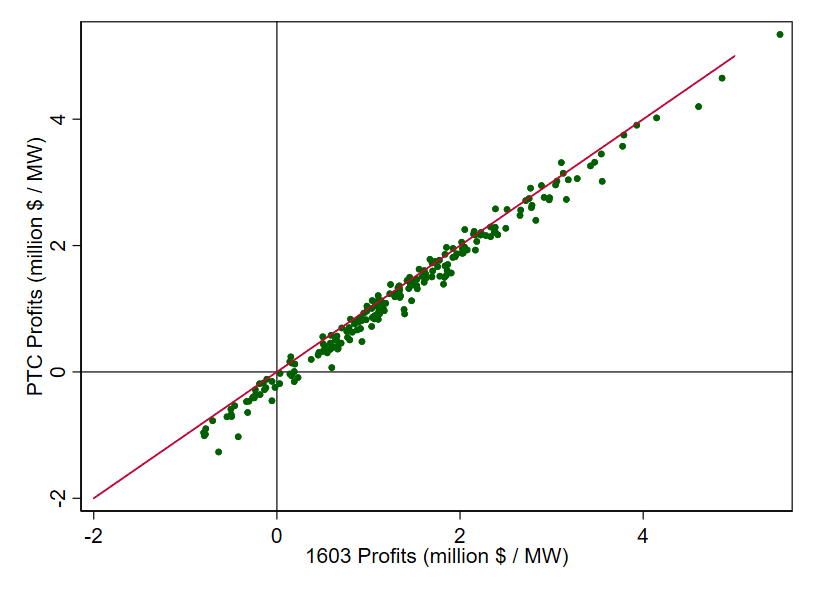
\includegraphics[width=0.75\linewidth]{../output/figures/1603_vs_PTC_pi_scatter.png}
\end{center}
\end{figure}

Figure~\ref{fig:1603_vs_PTC_scatter} presents a scatter plot of these two profit measures for plants selecting the 1603 grant. The 45-degree line reflects parity between the two, and, unsurprisingly, most plants selecting the investment subsidy earn less money under the output subsidy. Despite this, the graph also makes clear that the difference in profitability across plants within subsidy type is an order of magnitude larger than the difference across subsidies within a plant. And, since the distribution of plants is not particularly dense near the origin, very few plants appear marginal to the 1603 grant program. Of the \input{../output/estimates/N_CostEffectiveness_1603.tex} \unskip 1603 recipients included in this figure, only \input{../output/estimates/pe_baseline_pi-1603-only_N.tex} \unskip lie in the lower right quadrant.\footnote{This sample differs slightly from the sample used in Section \ref{sec:Empirical-Strategy} because we exclude plants with no price data and include plants who were omitted from the regression analysis due to missing wind speed data.} 

Estimating the full effect of the 1603 program on output requires taking a stand on the counterfactual entry status of the \input{../output/estimates/pe_baseline_pi-never_N.tex} \unskip plants in the lower left quadrant, which do not appear profitable under either subsidy. One possibility is to assume that these plants are in fact marginal, and would not have entered without the 1603 grant program. Under this assumption, the 1603 program increased lifetime wind production by \input{../output/estimates/pe_baseline_Marginal_dQ_diff.tex} \unskip million MWh, or \input{../output/estimates/pe_baseline_Marginal_dQ_diff_pct.tex} \unskip percent. In our view, this assumption is unlikely, given the graphical evidence on entry rates presented in Figure~\ref{fig:proposed_completed_on_time}. Instead, it seems more plausible that the apparent lack of profitability for these plants implies a policy-invariant unobservable (possibly in expectation) that would have encouraged these wind farms to enter with or without the 1603 grant.\footnote{There are many potential reasons why plants may appear unprofitable using this approach. We only observe a handful of years of output data, so our approach could understate the profits of wind farms that had low output realizations during the years we observe. We may have also underestimated state and local subsidies or overestimated O\&M costs and discount rates for some plants. However, even if we had perfectly accounted for all of these factors, it is likely that some plants that appeared profitable \emph{ex ante} will be unprofitable \emph{ex post} due to low price and wind realizations.} Under this assumption, the 1603 grant program \textit{reduced} production by \input{../output/estimates/pe_baseline_Always_dQ_diff.tex}million MWh. Additional results and sensitivity analysis are presented in Appendix \ref{Appendix:1603eval}.

\subsection{Cost-Effectiveness \label{sec:costEffectiveness}}

This paper addresses the question of cost-effectiveness of wind power subsidies: given some target level of wind energy, do input or output subsidies achieve it at lower cost? While the previous section compares output and entry under the 1603 grant program and the PTC, institutional details limit the ability of those analyses to provide a generic answer to this question. First, there are idiosyncratic tax code differences between the two policies. The PTC was implemented as a tax credit, which was more difficult to monetize, while accepting the 1603 grant precluded some accelerated depreciation \citep{johnston_nonrefundable_2019}. Second, wind developers were able to select between subsidy options, which, given the zero sum nature of the transfer, \emph{must} raise the public cost for some plants. Finally, given the significant heterogeneity in wind quality across locations, the marginal public cost likely varies across different output targets. In this section, we compute the total public cost per MWh of wind production over a range of output levels for each subsidy type, absent subsidy choice and differential tax treatment. 

Our starting point is the discounted profit functions under investment subsidy $s$ (equation \ref{eq:pi1603}) and output subsidy $\phi$ (equation \ref{eq:piPTC}). To gain intuition for which margin is more cost-effective, consider the case where all plants $i$ have the same output prices and investment costs, but differ in their productivity. Let $\bar{Q_i}$ be plant $i$'s discounted lifetime production, and, for the moment, assume output subsidies do not affect production, $\bar{Q_i}(\phi) = \bar{Q_i}$, conditional on operating. Plants enter if profits are positive, and, under these assumptions, the most productive plants enter first. We can arrange firms into an aggregate supply curve indexed by entry order $j$ with $\bar{Q}_{1} \ge \bar{Q}_{2} \ge ... \ge \bar{Q}_{N}$. Each plant has a breakeven investment subsidy $s^*_j$ and a breakeven output subsidy $\phi^*_j$.

Which subsidy is more cost-effective under these assumptions? Consider an output target that requires the first $J$ plants to enter. This can be achieved with breakeven $s^*_J$ or $\phi^*_J$. Since subsidies work at the margin, the total public subsidy paid to the $J$th firm must be the same across the two policies. However, since subsidies pay out across all inframarginal plants, the total subsidy paid across all $J$ firms will differ. The average output subsidy paid is greater than the marginal subsidy paid since inframarginal plants are more productive. Conversely, the average investment subsidy paid per plant is the same as the marginal subsidy paid, since all plants have the same investment costs. This is the insight of \citet{parish_relative_1982}: since investment is used more intensively at the margin than on average (it takes more investment per unit of output on the margin), investment subsidies will be cheaper. 

This result can be reversed by relaxing some of the assumptions made for ease of illustration. If other factors that positively affect entry, such as high output prices or low operating costs, are negatively correlated with plant productivity, then the marginal output per private dollar of investment need not decline as public subsidies increase. All else equal, the public cost-effectiveness of output subsidies (relative to investment subsidies) will improve if subsidy recipients produce more output when incentivized on the margin, as was estimated above. 

To calculate the net effect of these forces, we employ the accounting-based framework from the previous section. Starting with the no subsidy case, we determine the number of profitable entrants. We then incrementally increase subsidies up to the observed level of the 1603 and PTC subsidies, $s=0.3$ and $\phi=\$23$ per MWh. In the case of the output subsidy, we need to estimate the output firms would have produced under marginal incentives that are smaller than those observed in the data. Since the level of the PTC does not vary in our sample, it is not possible to directly estimate how output varies with the subsidy level. Instead, to approximate output under intermediate levels of the output subsidy, we scale our estimated output effect linearly. For example, the effect of an output subsidy of \$11.50 per MWh, half the value of the PTC, would be half our estimated output effect. As a result, changing the level of the subsidy affects plant profitability through both the level of the subsidy and the quantity of output. For each subsidy level, we compute total discounted output, government expenditures, and the public levelized cost of energy (LCOE) for plants that are profitable at that subsidy level. This allows a direct comparison of the alternative subsidies: to minimize the public expenditure needed to reach a certain quantity of output, the government can choose whichever subsidy achieves that level of output at lower public LCOE.

We begin by restricting our analysis to plants that selected the 1603 grant, as in the previous section. Figure \ref{fig:pub_lcoe_1603} presents the public cost per MWh of wind subsidized by subsidy type. Over \input{../output/estimates/ce_nosubsidy_dQ.tex} \unskip million MWh of wind enter without any subsidy.\footnote{This includes 1603 plants that are classified as never profitable.} To increase wind production, the public cost under investment subsidies rises faster than the cost of output subsidies. An output subsidy of $\phi = \$ \input{../output/estimates/ce_1603equivalentPTC_phi.tex}$/MWh results in the same total quantity of wind power as the 1603 investment subsidy rate of $s=0.3$. At this level, the public LCOEs are $\$ \input{../output/estimates/ce_1603_plcoe.tex}$/MWh and $\$ \input{../output/estimates/ce_1603equivalentPTC_plcoe.tex}$/MWh, for a $\input{../output/estimates/ce_1603equivalentPTC_plcoe_pct.tex}$ percent reduction in cost per MWh under the PTC.\footnote{Note that these public LCOEs are lower than Table \ref{tab:policyeval}, which includes accelerated depreciation.} To unpack this result, we also include public LCOE under the assumption that plant output is not affected by the subsidy margin. Here the two policies appear equally costly, highlighting that it is really the intensive margin response, rather than selection, driving the previous result. It is also noteworthy that the relative gains from output subsidies increase as the policy becomes more ambitious. As output subsidies grow to screen in increasingly less productive plants, they also induce greater effort at inframarginal plants. 

\begin{figure}[htbp]
\caption{Public LCOE vs Output by Subsidy Type}
\begin{center}%\centering
\begin{subfigure}[b]{0.495\textwidth}
	\caption{1603 Recipients \label{fig:pub_lcoe_1603}}
	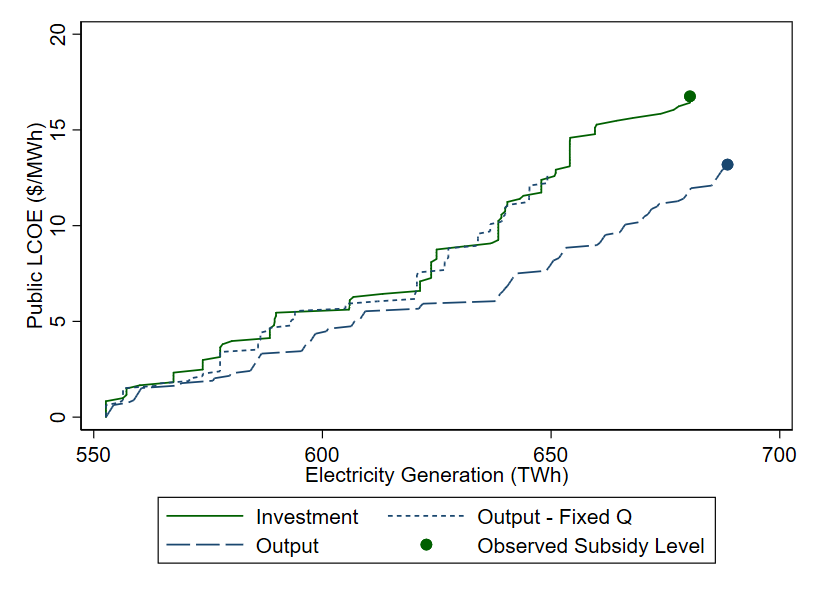
\includegraphics[width=\textwidth]{../output/figures/plcoe_plot_1603plants.png}
\end{subfigure} \hfill
\begin{subfigure}[b]{0.495\textwidth}
	\caption{All Plants \label{fig:pub_lcoe_all}}
	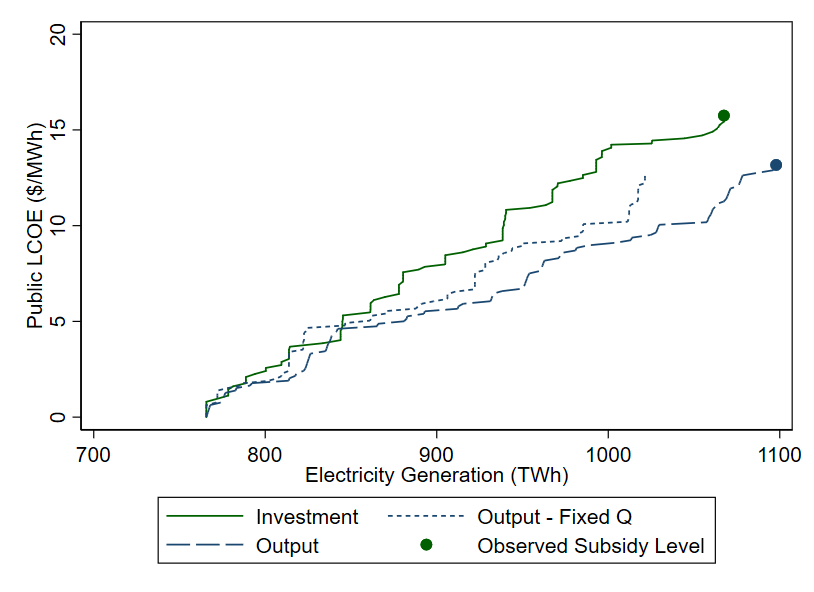
\includegraphics[width=\textwidth]{../output/figures/plcoe_plot_all.png}
\end{subfigure}
\end{center}
\vspace{-15pt}
\footnotesize
Each line plots the average public subsidy per unit of wind generation (LCOE) as a function of the total amount of wind generation subsidized. These are constructed by gradually increasing the subsidy from zero to the observed subsidy rates of the 1603 grant (investment) and PTC (output) subsidies. For output subsidy levels inframarginal to the PTC, we scale the estimated impact of the PTC on production linearly. For comparison, the ``Output - Fixed Q'' line plots the LCOE under the assumption that output is subsidized, but that this increase in marginal incentives does not affect plant productivity, conditional on operating. Panel (a) restricts the set of potential entrants to those selecting the 1603 grant, while panel (b) includes all wind farms entering between 2009 and 2012. In both figures, plants which are not marginal to either subsidy over the relevant range are assumed to always enter. The total output of these plants is reflected in the X-intercept of each figure. 
\end{figure}

Next we consider the cost-effectiveness of input and output subsidies without subsidy choice, incorporating plants that selected the PTC as well.\footnote{Estimating profits for PTC recipients is complicated by the fact that the government does not track investment costs for these firms. We compile cost information from a variety of sources, including SNL Energy, Bloomberg New Energy Finance (BNEF), state tax filings, regulatory filings and press releases. For the remaining plants, we predict missing costs using regression. Additional details provided in Appendix \ref{Appendix:CostEffectiveness-calculation-detail}.} Figure \ref{fig:pub_lcoe_all} presents the public LCOE over the range of output observed under inframarginal subsidies. The pattern is similar to the 1603 only sample, although the cost is noticeably lower under output subsidies even without any sort of productivity response. For this full sample, an output subsidy of $\phi = \$ \input{../output/estimates/ce_1603equivalentPTC_phi_allplants.tex}$/MWh results in the same total quantity of wind power as the 1603 investment subsidy rate of $s=0.3$. At this level, the public LCOEs are $\$ \input{../output/estimates/ce_1603_plcoe_allplants.tex}$/MWh and $\$ \input{../output/estimates/ce_1603equivalentPTC_plcoe_allplants.tex}$/MWh, which is also a $\input{../output/estimates/ce_1603equivalentPTC_plcoe_pct_allplants.tex}$ percent reduction.

In addition to all of the assumptions embedded in this accounting approach, it is important to acknowledge a few caveats. First, it's possible that achieving a more ambitious target or implementing the policy in future years could result in a positive correlation between productivity and other factors that positively affect entry, reversing the cost-effectiveness ordering. Furthermore, if investment subsidies were made permanent, project characteristics (which we have conditioned on) could respond. Investment subsidies like the 1603 grant are an example of a non-uniform input subsidy. Certain capital inputs, most notably wind turbines, were subsidized, while other inputs, like land, were not. When faced with a shift in the relative price of inputs, firms will likely alter their input mix, either by employing relatively more subsidized inputs or by selecting higher quality subsidized inputs \citep[as found for other industries in][]{goolsbee_taxes_2004}. Whether this input response increases or decreases public cost-effectiveness depends on the substitutability of inputs and the elasticity of output with respect to inputs at the margin \citep{parish_relative_1982}. However, such distortions are clearly socially inefficient. Unfortunately, the short lifetime of the 1603 program limits our ability to draw conclusions about how the capital stock would adjust to a permanent policy change.

\section{Conclusion \label{sec:Conclusion}}

The economically efficient response to the problem of pollution externalities from energy generation is to impose a Pigouvian tax on emissions, not to subsidize emissions-free production. Nevertheless, the use of both investment and output subsidies for green energy is widespread. For example, in the United States, the Federal government subsidizes solar energy through the Investment Tax Credit. At the same time, 33 states offer residential solar adopters some form of ``performance-based incentive'' (PBI), which pays above private marginal value for each unit of solar output.\footnote{Source: \href{https://www.solarpowerrocks.com/affordable-solar/what-are-solar-performance-payments-srec-pbi/}{https://www.solarpowerrocks.com/affordable-solar/what-are-solar-performance-payments-srec-pbi/}, accessed 7/10/2019. These take the form of feed-in tariffs, performance premiums, and solar renewable energy certificates.} In the European Union, 21 countries subsidized qualifying renewables using feed-in tariffs (payments per unit energy delivered to the grid), while seven offered investment grants or tax credits \citep{JENNER2013385}. 

In this paper, we exploit a natural experiment to directly estimate the relative cost-effectiveness of using output versus input subsidies to promote wind energy. We find that by removing subsidies for output on the margin, the Section 1603 grant program caused wind farms to generate \input{../output/estimates/stat_rd_estimate_pct.tex} \unskip to \input{../output/estimates/stat_match_estimate_pct.tex}percent less power than they would have under the PTC. Using firm-specific data on production, output prices, and investment costs, we find that very few plants appear profitable under one subsidy type but not the other. After standardizing the tax treatment of these subsidies and accounting for extensive margin effects, we show that output subsidies are more cost-effective over a large range of output targets. As an example, we find that the amount of wind power procured by a 30 percent investment subsidy could be achieved at $\input{../output/estimates/ce_1603equivalentPTC_plcoe_pct_allplants.tex}$ percent lower cost using an equivalently tax advantaged output subsidy.

What are the lessons for subsidies outside of energy policy? Investment subsidies are observed in several important settings where the social benefits of investment appear to be tied to output, such as affordable housing and research and development. The relative cost-effectiveness of output subsidies in these settings will depend on the production primitives of those markets, and we make no claim that our results are informative about optimal targeting in those domains. Nevertheless, the fact that investment subsidies appear poorly targeted in this setting should motivate future empirical work in other settings.

\pagebreak
\begin{singlespace}
\bibliographystyle{mychicago}
\bibliography{1603_all}
\end{singlespace}

%%%%%%%%%%%%%%%%%%%%%%%%%%%%%%%%%%%% APPENDIX %%%%%%%%%%%%%%%%%%%%%%%%%%%%%%%%%%%%%%%%%%%%%%%%%%%%%%%%%%%%%%%%
\appendix
\makeatletter
\def\@seccntformat#1{\csname Pref@#1\endcsname \csname the#1\endcsname\quad}
\def\Pref@section{Appendix~}
\makeatother

\counterwithin{figure}{section}
\counterwithin{table}{section}


\clearpage
\section{Data Appendix \label{sec:Data_Appendix}}

\subsection{Additional Information on Data Sources and Cleaning}

Information on how to obtain each data source, along with code for replication is available on \href{https://github.com/rlsweeney/public_ags_output_subsidies}{https://github.com/rlsweeney/public\_ags\_output\_subsidies}. 

\paragraph{Additional Information on the Primary Data Sources }
\begin{itemize}
\item \href{https://www.eia.gov/electricity/data/eia860/}{Survey Form EIA-860} collects generator-specific information on an annual basis about existing and planned generators and associated environmental equipment at electric power plants with 1 megawatt or greater of combined nameplate capacity.
\item \href{https://www.eia.gov/electricity/data/eia923/}{Survey Form EIA-923} collects detailed electric power data\textemdash with both monthly and annual frequency\textemdash on electricity generation, fuel consumption, fossil fuel stocks, and receipts at the power plant and prime mover level.
\item \href{https://www.awea.org/windiq}{The American Wind Energy Association (AWEA)} collects detailed information about all of its members and makes these data available as part of its membership subscription. The database includes more than 60 fields. We use the data to determine the presence and terms of any power purchase agreements and to construct a measure of the footprint of each wind farm.
\item \href{https://www.vaisala.com/en/industries-innovation/renewable-energy-and-weather}{3TIER windspeed data} provides hourly estimated wind speed data from 2000 to 2014 for every wind farm in the EIA database. We use these hourly data to compute the variance and a polynomial in observed wind speed, as well as the potential capacity factor, for each month.\footnote{These data were provided by Joern Huenteler, Gabe Chan, Tian Tang, and Laura Diaz Anadon, collected as part of their research summarized in \citet{huenteler_why_2018}. A handful of EIA plant locations were either entered erroneously or downloaded improperly, and are excluded from the sample.}
\item \href{https://www.treasury.gov/initiatives/recovery/Pages/1603.aspx}{The Department of the Treasury} reports data on Section 1603 grant claims. We matched Treasury Section 1603 grant projects to EIA data based on business name, plant name, county and state identifiers, and date placed in service. For 152 Section 1603 grants, we could not identify a match in the EIA data. One of these is a Puerto Rico project, which is excluded due to geography from the EIA databases. The other 151 projects received very small grants, indicating that these projects were too small to be covered by EIA's EIA-860 and EIA-923 surveys. In aggregate, they represent one-half of one percent of 1603 grant outlays for large wind projects. 

A grant could be submitted for a single wind turbine, a set of turbines, or an entire wind farm. This created two data issues. First, a wind farm could receive multiple Section 1603 grants. In these cases, we aggregated 1603 grants to the wind farm level (the level of observation in the EIA databases). For example, the large Alta wind farm in California came online in phases starting in late 2010 and its developers submitted more than twenty 1603 grants. Second, a wind farm could be built with N turbines that come online before 2009, for which it claims the PTC. It may then expand with M turbines in 2009 and claim a 1603 grant for these new turbines. The EIA-observed output for that wind farm after 2009 would reflect the aggregate production of the N+M turbines. Since we cannot distinguish the output between the N PTC-claiming turbines and the M 1603 grant-claiming turbines at such a wind farm, we drop the wind farm from our sample. We identified such cases as wind farms that claimed a 1603 grant over 2009-2012, but had either substantial pre-2009 generation or a significant change in installed capacity post-2012. Using these decision rules, we dropped thirteen wind farms that represent less than four percent of total 1603 grant outlays for large wind farms. 
\end{itemize}

\paragraph*{Additional Sample Restrictions}

There are 941 wind farms in the continental U.S. in the EIA data. We restrict attention to plants that are private and operate as either independent power producers or part of an investor-owned utility based on subsidy eligibility, which reduces the sample to 817 wind farms. We also restrict the sample to plants entering before the end of the 1603 grant period (end of 2012). There are two ways of determining when a plant is placed into service using the EIA data: we could use either the date a plant submits to the EIA as their first date of commercial operation or the month that a plant's production first appears in the production data. Conversations with EIA staff confirm that the former should be used for determining 1603 grant eligibility. However, to avoid concerns about potential misclassification, we exclude plants whose two entry dates suggest conflicting 1603 eligibility status. Finally, we exclude plants that we were unable to locate in the AWEA database, plants for which we did not have site-specific wind and turbine power curve information, and plants for which the ratio of observed capacity factor to potential capacity factor was further than two standard deviations from the median. This final sample of 512 plants represents our population.

\subsection{Potential Capacity Factor Construction \label{Appendix:Potential-capacity-factor}}

As described in Section~\ref{subsec:WindEcon}, wind farm production is a nonlinear function of wind speed. This nonlinear function is turbine-specific, as some turbines are engineered to perform particularly well at low wind speeds, while others are optimized for high wind speeds. Wind turbine manufacturers provide power curves for each turbine that summarize how much electricity it should generate at a given wind speed. Figure~\ref{fig:GE-powercurve} presents example power curves for two of the most common wind turbines in the U.S. The Vestas turbine has a higher maximum capacity, but the GE turbine is rated to produce power at higher wind speeds. Other turbines are designed to generate more electricity at lower wind speeds at the expense of generating less electricity at higher speeds.

\begin{figure}[h]
\caption{Reported Power Curves for Two Common Turbines \label{fig:GE-powercurve}}
\centering{}\includegraphics[width=0.7\textwidth]{../images/powercurve_ge_vestas.png}
\end{figure}

Rather than try to approximate this function with turbine-specific high order polynomials of wind speed, we compute an ``engineering'' estimate of expected output for each turbine in each month. We begin with estimates of the wind speed every hour at every wind farm in our sample that come from 3TIER. We combine this with a location-specific power function based on the wind turbine used at each wind farm to predict hourly electricity generation. We use the ideal gas law to adjust for variation in air density, which affects the kinetic energy available to each turbine, using location- and time-specific data on temperature and pressure from 3TIER. Aggregating hourly predicted output over the month and dividing by the turbine's rated output provides us with a measure of ``potential capacity factor,'' which we include as a covariate in our primary specifications.

Table~\ref{tab:wind_selection} demonstrates that this one-dimensional, time-varying control explains significantly more of the observed variation in capacity factor than time-invariant, site-specific wind quality information. It also fits meaningully better than a third order polynomial in wind speed.

\begin{table}[H]
\caption{Explanatory Power of Alternative Measures of Potential Generation \label{tab:wind_selection}}
\footnotesize
\begin{center}
\input{../output/tables/wind_covar_justification.tex}
\end{center}
Results from linear regressions of observed capacity factor on functions of wind speed data from EIA and 3TIER, using data on electricity generation in 2013 and 2014 for wind farms that came online between 2005 and 2012.
\end{table}



\clearpage
\section{Negative Prices and Emissions Rates \label{Appendix:NegativePrices}}

As was discussed in Section~\ref{sec:Mechanism}, there are two possible mechanisms through which an output subsidy can increase wind production: a dispatch effect when wind is at or near the margin, and an availability effect when wind is inframarginal. Under the assumption that the true marginal cost of dispatch in any given hour is zero, the frequency of negative prices provides an upper bound on the share of hours during which former channel could operate. In this appendix, we present summary statistics on the prevalence of negative prices during our sample period. We then correlate these moments with marginal emissions and damages estimates from the literature to assess whether wind output actually provides positive net benefits during periods when the dispatch effect operates. 

We collect high-frequency price data at multiple locations from six large U.S. electricity markets: California (CAISO), Texas (ERCOT), the Eastern U.S. (PJM), the Midwest (MISO), New England (ISONE), and New York (NYISO). Table~\ref{tab:Frequency-of-Negative} summarizes the likelihood of negatives prices in these six markets. The first panel contains summary statistics for all nodes (i.e., locations), and the second panel contains summary statistics for the set of nodes that are closest to each wind farm in our sample. Within the set of nodes near wind farms, negative prices are more common in California, Texas, and the Midwest. They are also less common in the summer, when demand is higher, and have generally been coming down over this sample period. Comparing across the two panels, negative prices are more common at nodes near wind farms than across all nodes in each ISO, although the difference varies considerably.

\begin{table}[h]
    \caption{Frequency of Negative Prices in Six ISOs (2011-2014)\label{tab:Frequency-of-Negative}}
    \vspace{-15pt}
    \footnotesize
    \input{../output/tables/negative_price_summary.tex}
    
    Frequencies (in percentage points) based on hourly nodal price data from the six listed ISOs, collapsed to the node-month level. Summer months are defined by the NOx regulation season, when begins in May and ends in October. In the second Section, the sample is restricted to nodes that are the closest node to a wind farm in the sample. The third Section of the table presents the average marginal operating emissions rate in pounds of carbon dioxide per MWh estimated for each ISO by \citet{callaway_location_2018}. The second row re-weights the average by the share of negative prices in each ISO-season-hour. The final row presents the correlation between negative prices and marginal operating emissions rates across 48 season-hour averages for each ISO.
\end{table}

We augment the negative price data with marginal operating emissions rates from \citet{callaway_location_2018}. \citet{callaway_location_2018} provide estimates of the average marginal operating emissions rate of generating resources by hour of day and season for each ISO, which we replicate in the first panel of Figure~\ref{fig:moer_np_season}. The second panel contains the frequency of negative prices for the same hours and seasons. Electricity prices typically fall below zero when demand is lowest, during the middle of the night. However, for four of the six ISOs, marginal emissions are actually \emph{higher} at night than during peak hours. This is not surprising due to the fact that natural gas is likely to be on the margin during the day, whereas coal is more likely to be on the margin at night. Comparing across the seasons, average emission rates are fairly constant, compared to the variation in negative price frequency.

\begin{figure}[H]
\caption{Marginal Emissions and Negative Price Frequency by Hour of Day and Season \label{fig:moer_np_season}}
\vspace{-25pt}
\begin{center}
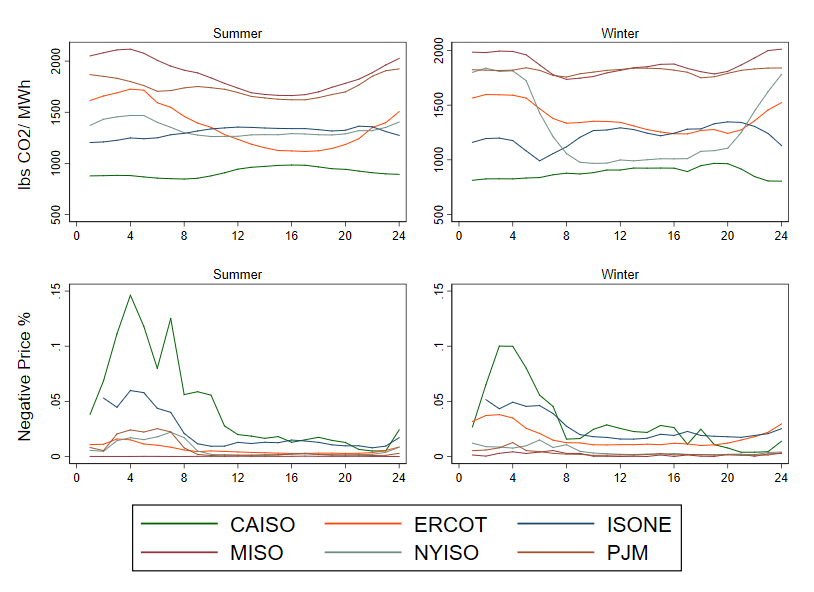
\includegraphics[width=0.75\textwidth]{../output/figures/moer_np_season.png}
\end{center}
\vspace{-15pt}
\footnotesize
Estimates of marginal operating emissions rates by hour of day and season were extracted from the appendix of \citet{callaway_location_2018}. Figures in the second row plot the mean share of negative price hours by ISO for the same hours and seasons. %
\end{figure}


The third panel of Table~\ref{tab:Frequency-of-Negative} contains average marginal emissions rates for each ISO. These emissions rates vary across regions, but are still positive and large everywhere, even when weighted by the negative prices in each ISO-season-hour. Finally, we present the correlation between negative prices and marginal operating emissions rates in the last row of Table~\ref{tab:Frequency-of-Negative}. In four of the six electricity markets, negative prices are positively correlated with marginal operating emissions rates, suggesting that the \textit{external} social value of wind energy during these hours is at least as high as during other time periods.

Finally, Figure~\ref{fig:md_np_hmmy} presents estimates of the average marginal damages from electricity generation in monetary terms from \cite{holland_are_2016}. These numbers include damages from both local and global air pollution. These estimates suggest that marginal damages are equal to or larger than the nominal value of the PTC in most regions and hours when averaged over all days of the year.

\begin{figure}[ht]
\begin{center}
\caption{Marginal Emissions Damages by Hour of Day \label{fig:md_np_hmmy}}
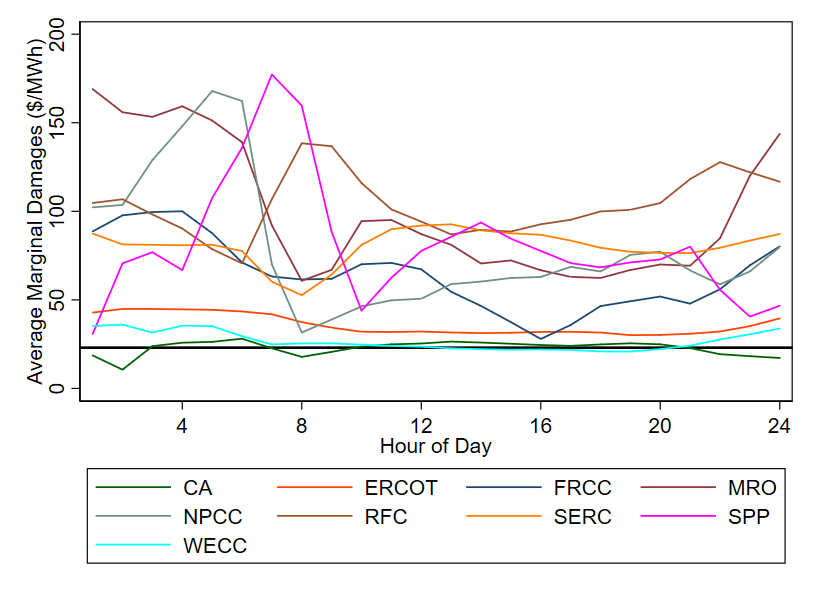
\includegraphics[width=0.75\textwidth]{../output/figures/md_np_hmmy.png}
\end{center}
\footnotesize Estimates of external marginal damages from electricity generation by hour of day and NERC region are taken from the replication materials for \citet{holland_are_2016}. The horizontal line is the nominal value of the PTC (\$23/MWh).
\end{figure}


\clearpage
\section{Profit Calculation Details \label{Appendix:Profitability-calculation-detail}}

Sections \ref{subsec:Extensive} and \ref{sec:costEffectiveness} approximate plant entry decisions using estimates of projected discounted profits under both subsidy regimes. These profit calculations require making assumptions about lifetime production, prices, operating costs, and discount rates. This appendix discusses each of these assumptions and presents additional sensitivity analysis.

The starting point for these calculations is two estimates of discounted lifetime profits for each plant given by:

\begin{align*}
\pi_i^{1603}&=\sum_{t=1}^{t=25} \left(\frac{p_{it}}{(1+r)^{t}}\right) Q_{it} - \frac{c_{it}}{(1+r)^{t}} -(1-s)F_i \\
\pi_i^{PTC}&=\sum_{t=1}^{t=25}\left(\frac{p_{it}}{(1+r)^t} + \frac{\phi_{it}}{(1+r^{tax})^t} \right) Q_{it}(\phi_{it}) - \frac{c_{it}}{(1+r)^t} - F_i
\end{align*}

\paragraph*{Time Horizon}
Plants are assumed to remain in service for 25 years, and right-censored prices and quantities are imputed with the observed (real) averages for each plant.

\paragraph*{Output Prices}

Plant-specific output prices ($p_{it}$) are computed using resale revenues reported on EIA Form 923, power purchase agreements from AWEA and BNEF, and estimated revenue from the sale of RECs.

Form EIA-923 began collecting annual resale revenue and quantity for each plant in 2011. The EIA refers to these data as ``resale,'' since the purchasing entity resells the power to end-use consumers. We infer average resale prices by dividing revenue by quantity and use this price for plants that sell all of their electricity for resale. For plants that report retail sales, we use average annual retail price information at the state level from Survey \href{https://www.eia.gov/electricity/data/eia861m/index.html}{EIA 861M}. In cases where firms report both types of sale, we construct a weighted average price. We exclude plants that are missing data on sales for resale and retail sales. We assume real prices remain at their current levels in future periods.

We also incorporate PPA data from AWEA and BNEF.  Both sources report multiple prices for some plants, and we use the median price for each plant from each source. We then take the maximum price derived from EIA resale data, AWEA resale data, and BNEF data as the price firms receive for their output in the electricity market.

Finally, we include estimated marginal revenue from the sale of RECs under state-level renewable portfolio standards using data from Marex Spectron and Lawrence Berkeley National Laboratory. As of 2017, 29 states and Washington D.C. had enacted RPSs. Wind farms generate certificates for each unit of production, which they then sell to utilities subject to the RPSs. Unfortunately, these payments are not observed in the EIA data.

We construct estimates of the RPS payments available to wind farms in a given state-month using bid-ask data on RECs trades from all active state RECs markets collected by Marex Spectron through May 2015. To account for the fact that some states allow covered non-renewable entities to obtain credits from qualifying renewable generators outside the state, we combine these state level prices with annual estimates of cross-state REC compliance flows from Lawrence Berkeley National Lab.\footnote{More information on this project tracking cross-state RECs at \href{https://emp.lbl.gov/projects/renewables-portfolio}{https://emp.lbl.gov/projects/renewables-portfolio}.} This expected REC payment is added to the average resale price to get marginal revenue each period. 

\paragraph*{Output Quantities}
Output under the 1603 ($Q_{it}$) is calculated based on the observed capacity factor. Output under the PTC ($Q_{it}(\phi_{it})$) is constructed by increasing observed capacity factor for each plant by \input{../output/estimates/stat_avg_estimate.tex} \unskip percentage points (reflecting the average of our preferred IV and matching results) for the first ten years of operation.

\paragraph*{O\&M Costs}
Plant-specific operations and maintenance costs ($c_{it}$) are unobserved, so we use \$29/kW/year (in 2018 dollars) for all plants based on \cite{wiser_2018_2019}.

\paragraph*{PTC Subsidy and Costs}
Under the PTC, firms receive $\phi_{it} = \$23$ additional dollars per MWh of output for first ten years of operation in the form of tax credits. Plants receive the full subsidy on inframarginal output that is generated under the 1603 ($Q_{it}$).

For additional electricity generated under the PTC, $Q_{it}(\phi_{it}) - Q_{it}$, O\&M costs should be higher on the margin than on average. Lacking plant-specific O\&M costs, we assume that plants receive half of the PTC subsidy value for marginal units. This is equivalent to assuming linear marginal costs for producing this marginal output, starting at zero and increasing to the level of the PTC.

\paragraph*{Fixed Costs}
Fixed investment costs ($F_i$) are obtained by dividing the observed 1603 grant award amount from Treasury by the fraction of investment costs covered by the program ($s=0.3$).

\paragraph*{Inflation Adjustment}
We put all revenues and costs in 2014 dollars. The PTC is indexed to inflation, so we use the 2014 value of \$23 per MWh for all PTC revenues. We observe other output prices (resale prices, PPAs, and RECs) and fixed costs ($F_i$) at different points in time for different projects. To put these prices in 2014 dollars, we follow the PTC inflation adjustment by using the GDP implicit price deflator from the U.S. Bureau of Economic Analysis.

\paragraph*{Discounting}
Output prices ($p_{it}$) and O\&M costs ($c_{it}$) are discounted at an assumed five percent real interest rate ($r$). The PTC subsidy ($\phi_{it}$) is discounted at a higher rate to account for the need to monetize tax credits discussed in Sections \ref{subsec:RenewablePolicies} and \ref{subsec:Extensive}. We use an eight percent interest rate ($r^{tax}$) because it is the modal tax equity yield over 2009-2012 presented in \citet{bolinger_analysis_2014}. We use the maximum observed tax equity yield of 10.5 percent for sensitivity analysis in Appendix \ref{Appendix:1603eval}.

\paragraph*{Accelerated Depreciation}
Wind farms were eligible for accelerated depreciation of fixed investment costs during the sample period. This can be viewed as an additional subsidy that may affect plant profitability. In addition, the value of accelerated depreciation depends on the subsidy firms choose: for 1603 recipients, the cost basis for depreciation is reduced by half the grant amount. This means that firms can depreciate 85 percent of the fixed cost under the 1603 versus 100 percent under the PTC.

While our focus is on the economic profits of wind farms rather than their financial structure and tax payments, the details of accelerated depreciation could affect plant profitability, plant subsidy choice, and government expenditures. To account for this, we compute the subsidy value of accelerated depreciation relative to straight line depreciation for each subsidy case. For accelerated depreciation, we first account for 50 percent bonus depreciation and then use the 5-year MACRS depreciation schedule from Table A-1 of the 2012 IRS Publication 946 for the remaining cost basis. For straight line depreciation, we depreciate the investment cost over the lifetime of production (assumed to be 25 years) and assume zero scrap value. We use the appropriate cost basis (85 percent or 100 percent of the investment cost) depending on the policy case. Depreciation flows are translated into dollars using a marginal tax rate of 35 percent and then converted to net present value using the assumed discount rate of five percent. Finally, we compute the subsidy value of accelerated depreciation by taking the difference between the depreciation ``revenues'' under these two schedules and adding that difference to plant profits. We also add that amount to the public expenditure to reflect the difference in tax receipts under the two subsidies.

\subsection{Section 1603 Program Evaluation \label{Appendix:1603eval}}

Table~\ref{tab:policyeval} summarizes these two constructed profit measures for 1603 grant recipients.\footnote{This sample differs slightly from the sample used in Section \ref{sec:Empirical-Strategy} because we exclude plants with no price data and include plants who were omitted from the regression analysis due to missing wind speed data.} The first two columns of the table report predicted lifetime output along with the total subsidy paid to 1603 claimants, both discounted using a five percent real interest rate.\footnote{Total government payments include accelerated depreciation benefits under each subsidy.} The third column presents the ratio of total subsidy to total output, which can be interpreted as the public LCOE. The final three columns present predicted output, subsidy, and public LCOE for these projects had they claimed the PTC instead of the 1603 grant. Plants are assigned to one of three groups: an always profitable group ($\pi^{1603}>0$ \& $\pi^{PTC}>0$), a marginal group ($\pi^{1603}>0$ \& $\pi^{PTC}<0$), and a never profitable group ($\pi^{1603}<0$ \& $\pi^{PTC}<0$).

Estimating the full effect of the 1603 program requires taking a stand on the counterfactual entry status of the never-profitable group. If these plants are in fact marginal, and would not have entered without the 1603 grant program, the 1603 program increased lifetime wind production by \input{../output/estimates/pe_baseline_Marginal_dQ_diff.tex}million MWh (\input{../output/estimates/pe_baseline_Marginal_dQ_diff_pct.tex} \unskip percent) while increasing the average public LCOE by $\$ \input{../output/estimates/pe_baseline_Marginal_lcoe_diff.tex} $/MWh (\input{../output/estimates/pe_baseline_Marginal_lcoe_diff_pct.tex} \unskip percent). If instead the never-profitable plants would have entered in either case, the 1603 grant program screened in just \input{../output/estimates/pe_baseline_pi-1603-only_dQ.tex}million MWh of production (in discounted terms) at the \input{../output/estimates/pe_baseline_pi-1603-only_N.tex}marginal plants. At the same time, production at inframarginal plants declined. Under this assumption, our preferred assumption, total wind output would have been slightly \emph{higher} without the 1603 program (by \input{../output/estimates/pe_baseline_Always_dQ_diff.tex}million MWh, or \input{../output/estimates/pe_baseline_Always_dQ_diff_pct.tex}percent). This would also imply that the 1603 grant increased the average public LCOE by $\$ \input{../output/estimates/pe_baseline_Always_lcoe_diff.tex} $/MWh (\input{../output/estimates/pe_baseline_Always_lcoe_diff_pct.tex} \unskip percent).

\begin{table}[H]
\caption{Estimated Subsidy by Group\label{tab:policyeval}}
\vspace{-15pt}
\input{../output/tables/policyevaltab_baseline.tex}
\footnotesize
Estimated electricity generation and subsidy for 1603 recipients, divided into three groups depending on their estimated profitability under the 1603 grant and the PTC. Output and Subsidy are in net present value terms, and Subsidy per MWh is constructed by taking the ratio of the sum of discounted subsidy expenditures to the sum of discounted electricity generation as in the definition of the LCOE. The first set of numbers correspond to outcomes under the subsidy they chose. The second set presents a counterfactual for the subsidy they did not choose.
\end{table}

Table \ref{tab:policyeval_highrtax} summarizes the results of the profitability calculation when using the maximum observed tax equity yield of 10.5 percent for $r^{tax}$ instead of the median yield of 8 percent. Under this alternative assumption, the number of always profitable plants decreases from \input{../output/estimates/pe_baseline_pi-always_N.tex} \unskip to \input{../output/estimates/pe_highrtax_pi-always_N.tex}\unskip, while the number of marginal plants increases from \input{../output/estimates/pe_baseline_pi-1603-only_N.tex} \unskip to \input{../output/estimates/pe_highrtax_pi-1603-only_N.tex}\unskip. As above, estimating the full effect of the 1603 program requires taking a stand on the counterfactual entry status of the never-profitable group. Under the assumption that never-profitable plants are in fact marginal, the 1603 program increased lifetime wind production by \input{../output/estimates/pe_highrtax_Marginal_dQ_diff.tex}million MWh (\input{../output/estimates/pe_highrtax_Marginal_dQ_diff_pct.tex} \unskip percent) and increased the public LCOE by $\$ \input{../output/estimates/pe_highrtax_Marginal_lcoe_diff.tex} $/MWh (\input{../output/estimates/pe_highrtax_Marginal_lcoe_diff_pct.tex} \unskip percent). If instead the never-profitable plants would have entered in either case, the 1603 grant increased the average public LCOE by $\$ \input{../output/estimates/pe_highrtax_Always_lcoe_diff.tex} $/MWh (\input{../output/estimates/pe_highrtax_Always_lcoe_diff_pct.tex} \unskip percent).

\begin{table}[H]
\caption{Estimated Subsidy by Group using $r^{tax} = 10.5\%$\label{tab:policyeval_highrtax}}
\vspace{-15pt}
\input{../output/tables/policyevaltab_highrtax.tex}
\footnotesize
Estimated electricity generation and subsidy for 1603 recipients, divided into three groups depending on their estimated profitability under the 1603 grant and the PTC. Output and Subsidy are in net present value terms, and Subsidy per MWh is constructed by taking the ratio of the sum of discounted subsidy expenditures to the sum of discounted electricity generation as in the definition of the LCOE. The first set of numbers correspond to outcomes under the subsidy they chose. The second set presents a counterfactual for the subsidy they did not choose.
\end{table}


\subsection{Modifications for Cost-Effectiveness Analysis\label{Appendix:CostEffectiveness-calculation-detail}}

For the cost-effectiveness analysis in Section \ref{sec:costEffectiveness}, we simplify our profitability calculations to focus on the core economic tradeoffs of input and output subsidies. The most prominent changes are summarized in the text, and the rest are summarized below.

\paragraph*{Fixed Cost Estimation for PTC Recipients}
Extending this analysis to PTC plants requires information on the investment costs of these plants. For 1603 plants, investment costs are observed because they are subsidized. For PTC plants, no such government information is available. To fill this gap, we collect plant-level investment costs from a variety of sources: SNL Energy, BNEF, state tax filings and press releases. Of the \input{../output/estimates/N_CostEffectiveness_PTC.tex} \unskip sample PTC plants entering between 2009 and 2012, we could not find cost information for \input{../output/estimates/N_CostEffectiveness_PTC_missing.tex} \unskip of these plants. 

We predict missing costs using a linear regression of costs onto plant characheristics for the plants whose costs we do observe. The sample is restricted so plants coming online within one year of the policy period (2008 - 2013). Cost are available for \input{../output/estimates/N_cost_regsample.tex} \unskip  plants during this period, \input{../output/estimates/N_cost_regsample_PTC.tex} \unskip of which claimed the PTC. Table \ref{tab:cost_prediction} presents the results. The dependent variable in each regression in the cost per unit of capacity (million \$/MW), and all models include plant vintage fixed effects. Model 1 shows that 1603 plants cost \$70,000 more per MW of capacity within cohort, although this estimate is not significantly different from zero. After controlling for plant size (model 2) and turbine firm and size (model 3), there is effectively no difference in costs between PTC and 1603 plants. After including state fixed effects in column 4, the root mean square error is \$270,000, which is approximately ten percent of the sample average cost. This final model is used for imputing missing plant costs in Section \ref{sec:costEffectiveness}.


\begin{table}[H]
\caption{Fixed Cost Estimation \label{tab:cost_prediction}}
\begin{center}
\input{../output/tables/cost_prediction.tex}
\end{center}
\footnotesize
The dependent variable in each regression is the upfront investment cost in million \$/MW. Sample restricted to plants entering 2008-2013 with non-missing investment costs. All models contain cohort (year of entry) dummies. Robust standard errors reported in parentheses.
\end{table}

\paragraph*{Omit Accelerated Depreciation}
We focus on economic profits and omit the subsidy value of accelerated depreciation described above.

\paragraph*{Discounting}
We abstract from the tax credit nature of the PTC and discount PTC revenues at the same rate as electricity revenues (i.e., 5 percent).


\clearpage
\section{Additional Tables and Figures}

\begin{table}[H]
\caption{Summary Statistics by Entry Date \label{tab:Summary-Statistics}}
\vspace{-15pt}
\input{../output/tables/annual_sum_stats.tex}
\footnotesize
Each row contains summary statistics for the set of wind farms in our sample that were placed into service in that year. Plants (all) is the number of wind farms placed into service in that year, Plants (sample) is the number in our restricted sample (see text and Appendix~\ref{sec:Data_Appendix}), and Plants (1603) is the number of Section 1603 grant recipients. All remaining columns are constructed using 2014 data from EIA Forms 860 and 923 except for Capacity and Turbine Size, which are constructed using the first values reported to the EIA. IOU or IPP is the share of wind farms that are owned by an investor-owned utility or independent power producer. Regulated is the share of wind farms that are regulated. Capacity is the average total nameplate capacity in MW. Turbine Size is the average turbine capacity in MW. Wind Speed is the average annual wind speed in miles per hour for each wind farm as reported to the EIA. Capacity Factor is the average of net electricity generation divided by capacity.
\end{table}

%\subsection{Linear RD Results \label{sec:LinearRD}}

\begin{table}[H]
\caption{IV Results Sensitivity: Linear RD \label{tab:rdd_cf_linear}}
\begin{center}{\footnotesize{}\input{../output/tables/rdd_regressions_cf_linear.tex}}\end{center}
\footnotesize
Data include a balanced panel of monthly observations from 2010 to 2014 for all wind farms. The first three columns replicate the IV results in Table~\ref{tab:rdd_cf}. For columns 4 - 6, distance to the policy cutoff, and that distance interacted with the a post-policy indicator are included as controls. All models contain year-month dummies. Standard errors clustered by wind farm reported in parentheses.
\end{table}


\begin{table}[h]
\caption{Matching Results Sensitivity: Matching on Potential Capacity Factor \label{tab:matching_group_ptnlcf}}
\begin{center}
\input{../output/tables/exact_match_state_ptnlcf.tex}
\end{center}
\footnotesize
The matched sample was constructed using coarsened exact matching on state, regulatory status, entity type, capacity, and potential capacity factor. All models include the controls listed in the IV models in Table~\ref{tab:rdd_cf}: log capacity, potential capacity factor, and wind speed variance, as well as dummies for whether the plant is regulated, whether it is an IPP, the presence of a PPA, and month of sample. All models also include cohort dummies. Standard errors, clustered at the plant level, are reported in parentheses.
\end{table}

\clearpage

%\subsection{Wind Farm Locations by Period and Subsidy}

\begin{sidewaysfigure}[h] \centering
	\caption{New Wind Farms by Subsidy (2009-2012)\label{map:2009to2012}}
	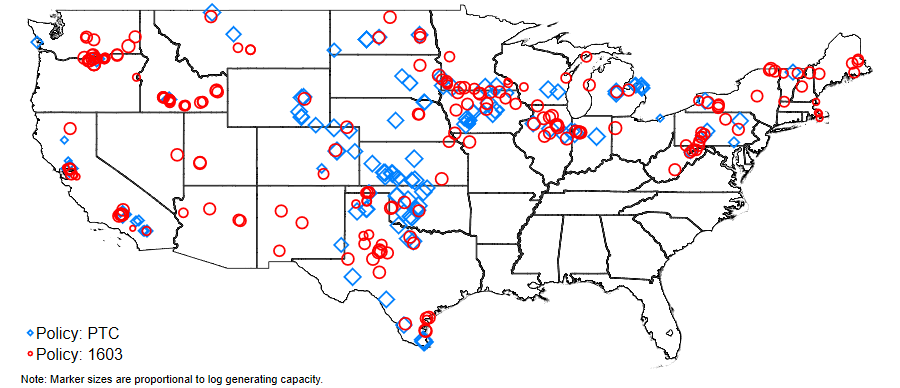
\includegraphics[width=\textwidth]{../output/figures/map_2009to2012.png}
\end{sidewaysfigure}

\begin{sidewaysfigure}[h] \centering
	\caption{New Wind Farms by Subsidy (2008-2009)\label{map:2008to2009}}
	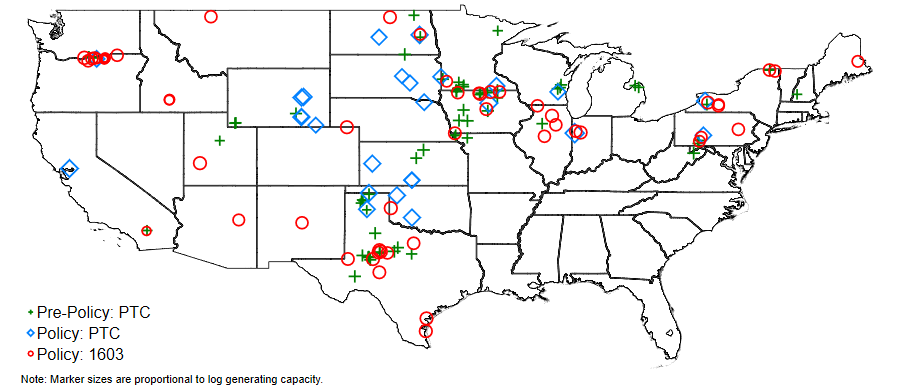
\includegraphics[width=\textwidth]{../output/figures/map_2008to2009.png}
\end{sidewaysfigure}

%\subsection{Additional Data on Power Plant Proposal and Completion}

\begin{figure}[h]
\caption{Share of Plants Ever Completed, Plotted by Year of Initial Expected Completion\label{fig:proposed_ever_completed}}
\vspace{-15pt}
\begin{center}
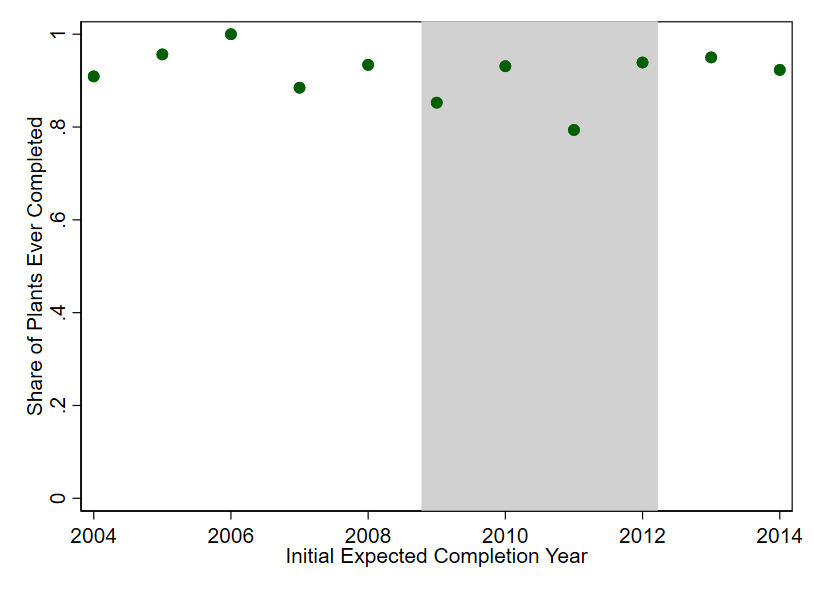
\includegraphics[width=0.75\linewidth]{../output/figures/proposal_data_ever_completed.png}
\end{center}
\vspace{-15pt}
\footnotesize
The initial expected completion year is the year the generator was first scheduled to start operation. Completion is determined based on when each plant entered into the EIA-860 operable data. Plots are based on the subset of plants that last appeared in the EIA-860 proposed data prior to 2016. Shading indicates the years during which new plants were eligible for the 1603 grant (2009 to 2012).
\end{figure}


\end{document}


%%%%%%%%%%%%%%%%%%%%%%%% UNUSED %%%%%%%%%%%%%%%%%%%%%%%%%%%%%%%%%%%%%%%%%%
% OLD MODEL:

\section{A Model of Subsidy Choice\label{subsec:model}}

Our analysis compares the productivity of plants that receive an output subsidy to those that receive an investment subsidy. The central empirical challenge our estimators address is the fact that subsidy assignment is selected. In this appendix, we present a simple model of subsidy selection, and show that selection depends on the product of (unobserved) productivity and prices. 

Consider a wind farm with $K$ megawatts of capacity that has already been constructed. In each time period, if the wind farm is available, it generates electricity and receives a price $p$ per unit of electricity. Availability, $a$, follows a Bernoulli distribution with success probability $\alpha$. Wind farms can influence this success rate through costly effort, $e$, exerted in advance at maintenance cost $m$ (both denoted per unit capacity). Effort is assumed to have decreasing returns, with $\alpha(e)'>0$, $\alpha(e)''<0$. Since effort is chosen in advance, availability realizations are independent of the realized price, $E[a|e,p]=E[a|e]=\alpha(e)$.\footnote{This assumes that wind farm availability and output have no impact on equilibrium prices. Given that wind farms are small relative to demand and that electricity markets are relatively well integrated, this is a reasonable assumption.} Per period operating profits are 
\begin{equation}
\pi_{0}=K[p\alpha(e)-me].\label{eq:capital_op_pi}
\end{equation}

At the start of each operating period, the firm selects $e$ to maximize expected operating profits. Its optimization program selects maintenance by equating the marginal cost of effort with the marginal induced change in availability times the expected price
\begin{equation}
E[p]\alpha'(e)-m=0.\label{eq:capital_foc}
\end{equation}
Denote this optimal effort level $e_{0}$ and the corresponding availability rate $\alpha_{0}$.

Now consider an output subsidy $s$ per unit of quantity produced. Expected operating profits per period become 
\begin{equation}
\pi_{1}=K[(E[p]+s)\alpha(e)-me],\label{eq:output_op_pi}
\end{equation}
with corresponding first order condition 
\begin{equation}
(E[p]+s)\alpha'(e)-m=0.\label{eq:output_foc}
\end{equation}
Denote this optimal effort level $e_{1}$ and the corresponding availability rate $\alpha_{1}$. Under the assumption that $\alpha''<0$ , the effort level with the subsidy ($e_{1}$) will be higher than without ($e_{0}$). This implies that, all else equal, expected output ($K\alpha$) will be higher with output subsidies as well. 

Now consider an alternative subsidy which reduces upfront capital costs $F$ by $\psi$ percent. Lifetime expected profits under this investment subsidy are 
\begin{equation}
\Pi_{0}=TK[E[p]\alpha_{0}-me_{0}]-(1-\psi)F,\label{eq:capital_Pi_total}
\end{equation}
where $T$ is the lifetime of a wind farm.\footnote{We do not explicitly include a discount factor for clarity, and instead subsume discounting into $T$.} At the start of operation, the firm must decide if it prefers those profits to the profits under the output subsidy, 
\begin{equation}
\Pi_{1}=TK[(E[p]+s)\alpha_{1}-me_{1}]-F,\label{eq:output_Pi_total}
\end{equation}
which is the case if 
\begin{eqnarray}
\psi(F/K) & > & T\left\{ (E[p]+s)(\alpha_{1}-\alpha_{0})-m(e_{1}-e_{0})\right\} +s T\alpha_{0}.\label{eq:selection}
\end{eqnarray}

For small changes in effort, the term in braces on the right will be zero under the envelope theorem, and equation~\ref{eq:selection} predicts that investment subsidies will be preferred by firms with high per unit capital costs ($F/K$) relative to their baseline (unsubsidized) expected operating level ($\alpha_{0}$). Intuitively, the inequality states that wind farms will prefer output subsidies when this additional operating profit is greater than the forgone subsidy per unit of capacity. For non-marginal changes in effort, the choice will also depend on the concavity of $\alpha$.

It is this correlation between subsidy preference and latent productivity which generates selection in subsidy choice and confounds our evaluation of the 1603 grant program. There are measures that wind farm operators can take that will increase output conditional on other attributes, as discussed in Section~\ref{subsec:WindEcon}. If these measures are costly, then increasing the marginal price received for output will make adoption more likely under the PTC. Thus, conditional on operating, we predict that removing the PTC will result in lower output. Ideally we would estimate $\tau=E[K_{i}(\alpha_{i0}-\alpha_{i1})]$. However, the policy was implemented with a choice, so we are only able to observe $\hat{\tau}=E[K_{i}\alpha_{i0}|\Pi_{i0}>\Pi_{i1}]-E[K_{i}\alpha_{i1}|\Pi_{i0}<\Pi_{i1}]$. 






